\documentclass[10pt, compress, aspectratio=169]{beamer}

\usetheme[numbering=fraction, progressbar=none, titleformat=smallcaps, sectionpage=none]{metropolis}
\usepackage{booktabs}
\usepackage{array}
\usepackage{listings}
\usepackage{graphicx}
\usepackage[english]{babel}
\usepackage[scale=2]{ccicons}
\usepackage{url}
\usepackage{relsize}
\usepackage{wasysym}

\usepackage{pgfplots}
\usepgfplotslibrary{dateplot}

\lstset{ %
  backgroundcolor={},
  basicstyle=\ttfamily\footnotesize,
  breakatwhitespace=true,
  breaklines=true,
  captionpos=n,
  commentstyle=\color{orange},
  escapeinside={\%*}{*)},
  extendedchars=true,
  frame=n,
  keywordstyle=\color{orange},
  language=C++,
  rulecolor=\color{black},
  showspaces=false,
  showstringspaces=false,
  showtabs=false,
  stepnumber=2,
  stringstyle=\color{gray},
  tabsize=2,
  keywords={thrust,plus,device_vector, copy,transform,begin,end, copyin,
  copyout, acc, \_\_global\_\_, void, int, float, main, threadIdx, blockIdx,
  blockDim, if, else, malloc, NULL, cudaMalloc, cudaMemcpy, cudaSuccess,
  cudaGetLastError, cudaDeviceSynchronize, cudaFree, cudaMemcpyDeviceToHost,
  cudaMemcpyHostToDevice, const, data, independent, kernels, loop,
  fprintf, stderr, cudaGetErrorString, EXIT_FAILURE, for, dim3},
  otherkeywords={::, \#pragma, \#include, <<<,>>>, \&, \*, +, -, /, [, ], >, <}
}

\renewcommand*{\UrlFont}{\ttfamily\smaller\relax}

\graphicspath{{../img/}}

\title{Autotuning High-Level Synthesis for FPGAs}
\author{\footnotesize Pedro Bruel \\ {\scriptsize phrb@ime.usp.br}}
\institute{
\includegraphics[height=2cm]{imelogo}\\[0.2cm] Universidade de São Paulo}
\date{\scriptsize September 15th 2016}

\begin{document}

\maketitle

\section{Introduction}

\subsection{About}

\begin{frame}
    \frametitle{About}
    \begin{columns}[T,onlytextwidth]
        \column{0.5\textwidth}
        \begin{center}
            
\includegraphics[width=.32\textwidth]{pedro}

            Pedro Bruel

            \textit{phrb@ime.usp.br}
        \end{center}

        \begin{center}
            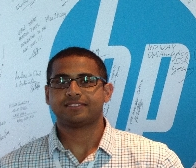
\includegraphics[width=.34\textwidth]{sai}

            Sai Rahul Chalamalasetti

            \textit{sairahul.chalamalasetti@hpe.com}
        \end{center}

        \column{0.5\textwidth}
        \begin{center}
            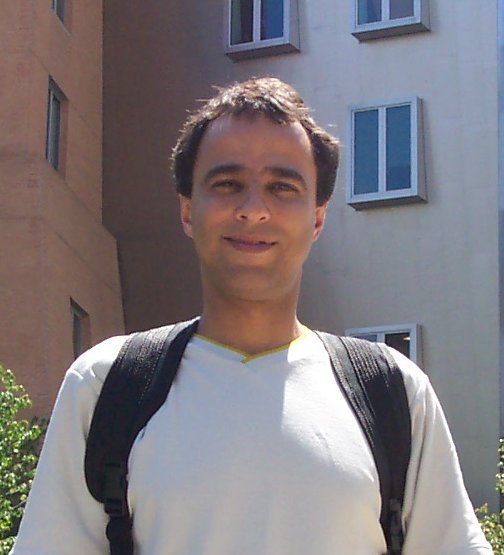
\includegraphics[width=.3\textwidth]{alfredo}

            Alfredo Goldman

            \textit{gold@ime.usp.br}
        \end{center}

        \begin{center}
            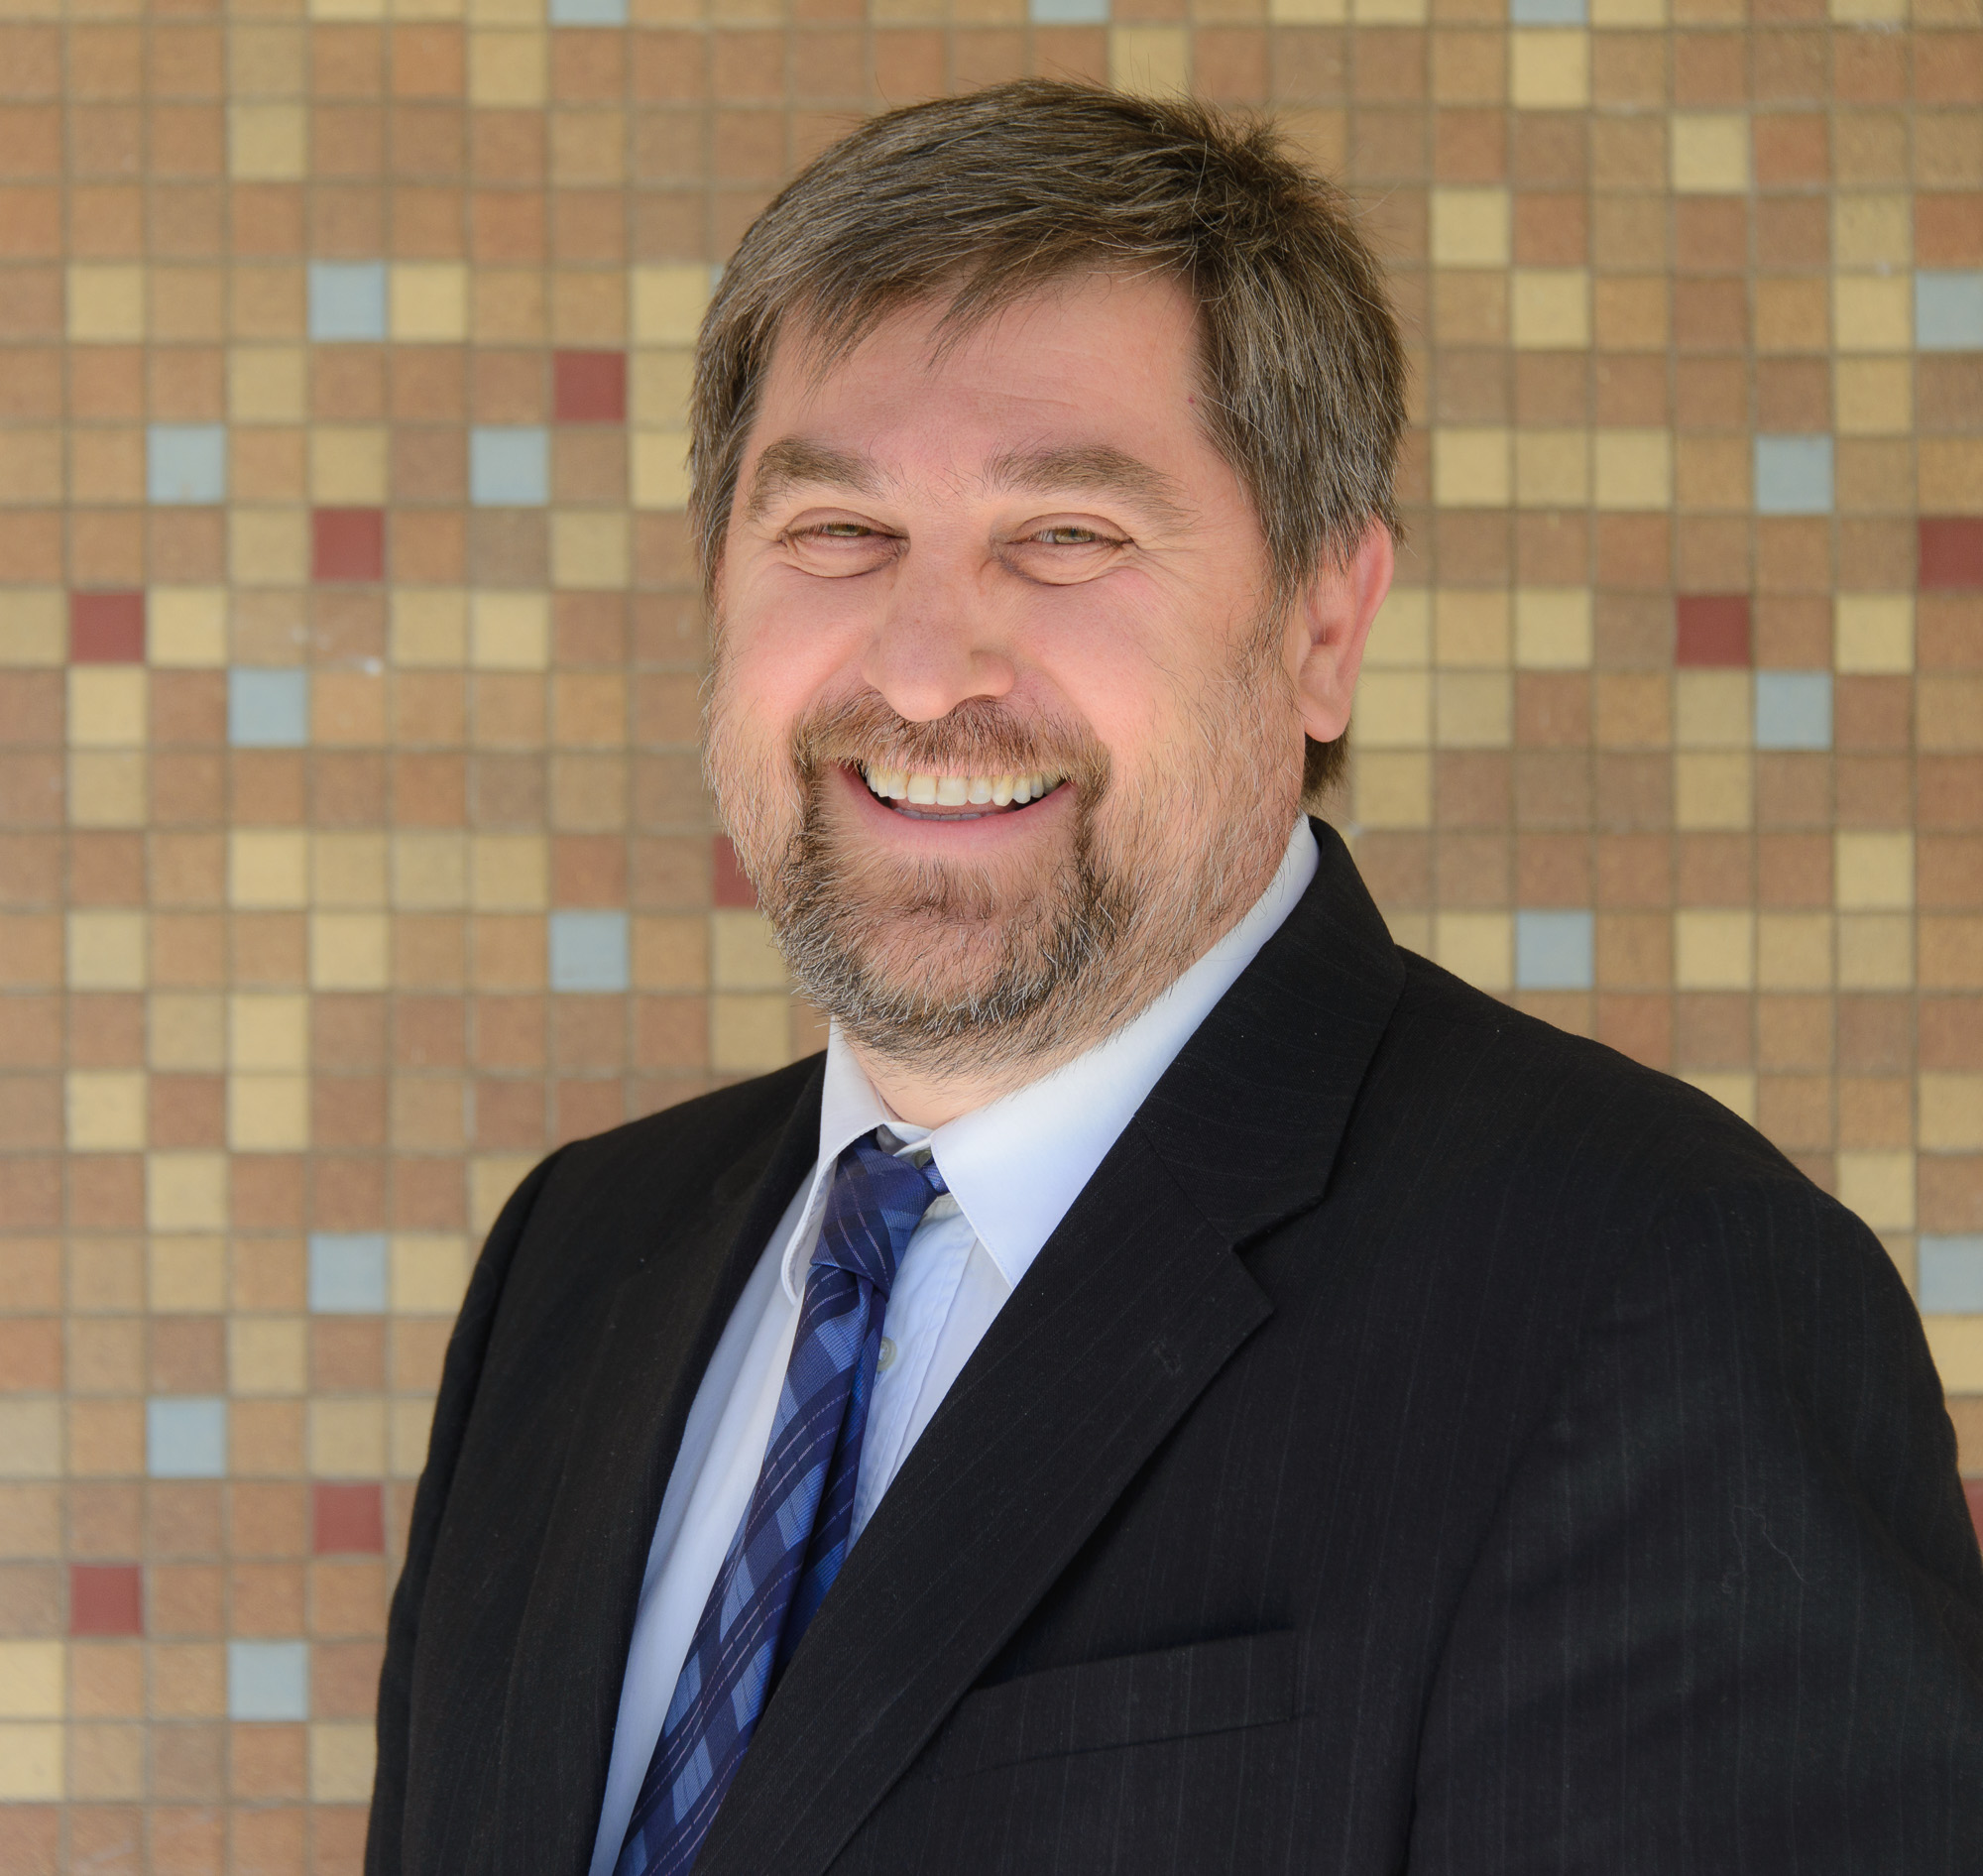
\includegraphics[width=.32\textwidth]{dejan}

            Dejan Milojicic

            \textit{dejan.milojicic@hpe.com}
        \end{center}

    \end{columns}
\end{frame}

\subsection{Field-Programmable Gate Arrays}

\begin{frame}
    \frametitle{Field-Programmable Gate Arrays (FPGAs)}
    \begin{columns}[c,onlytextwidth]
        \column{0.6\textwidth}
        FPGAs:
        \begin{itemize}
            \item \alert{Logic Blocks} and \alert{Interconnections}
            \item \alert{Reconfigurable}
        \end{itemize}

        Tradeoff:
        \begin{itemize}
            \item \alert{Energy Efficiency} and \alert{Performance}
            \item \alert{Programmability}
        \end{itemize}

        \column{0.4\textwidth}
        \begin{center}
            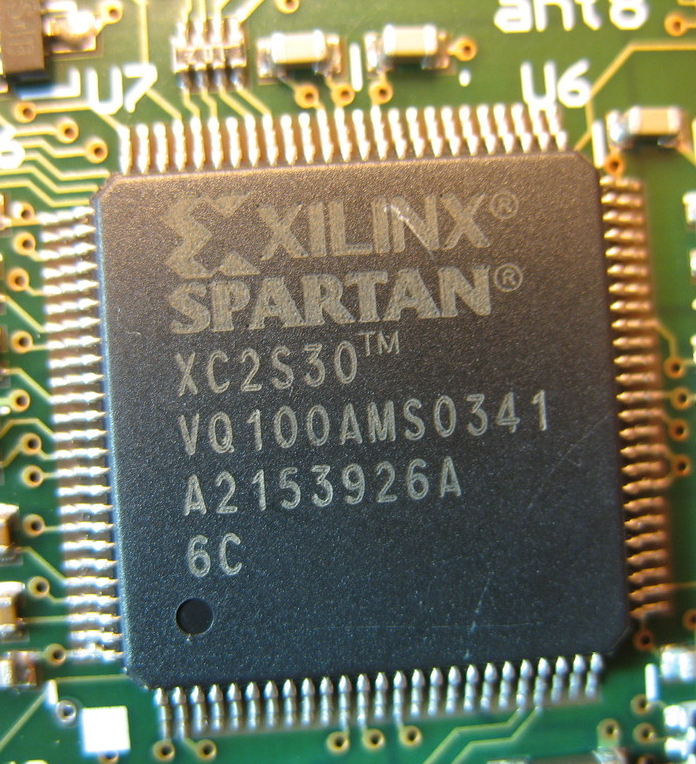
\includegraphics[width=.9\textwidth]{fpga}
        \end{center}
    \end{columns}
\end{frame}

\begin{frame}
    \frametitle{Field-Programmable Gate Arrays (FPGAs)}
    FPGAs used to speed up Bing search:
    \begin{center}
        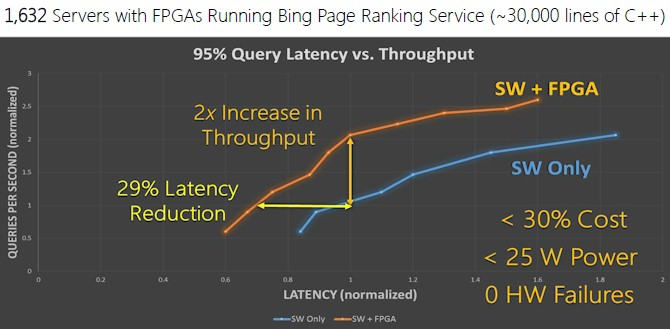
\includegraphics[width=.7\textwidth]{fpga_bing}

        \tiny{Image: \url{enterprisetech.com/2014/09/03/microsoft-using-fpgas-speed-bing-search/} [Accessed on 14/09/16]}
    \end{center}
\end{frame}

\subsection{High-Level Synthesis for FPGAs}

\begin{frame}
    \frametitle{High-Level Synthesis (HLS) for FPGAs}
    \alert{LegUp} HLS flow:

    \begin{center}
        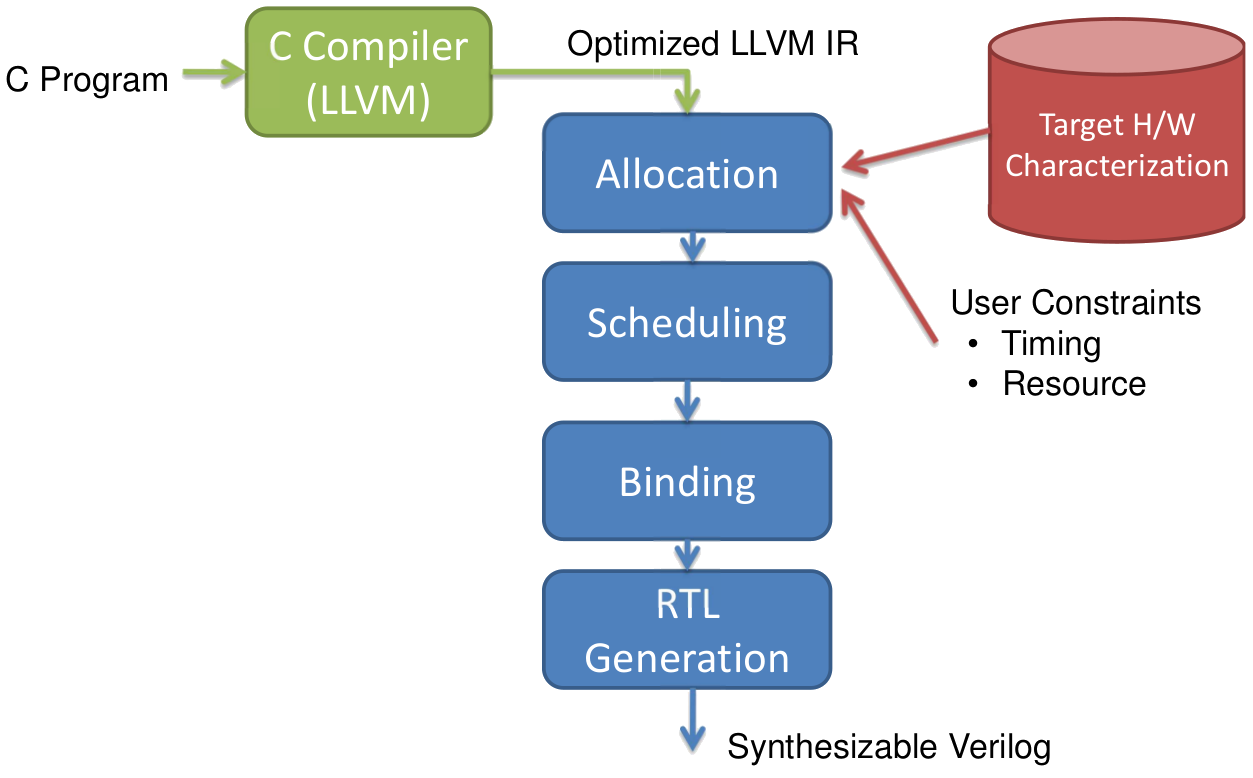
\includegraphics[width=.72\textwidth]{legup_flow}

        \tiny{Image: Canis, Andrew Christopher. LegUp: Open-Source High-Level Synthesis Research Framework. Diss. University of Toronto, 2015.}
    \end{center}
\end{frame}

\begin{frame}
    \frametitle{High-Level Synthesis (HLS) for FPGAs}
    HLS can generate \alert{lower-latency applications}:
    \begin{center}
        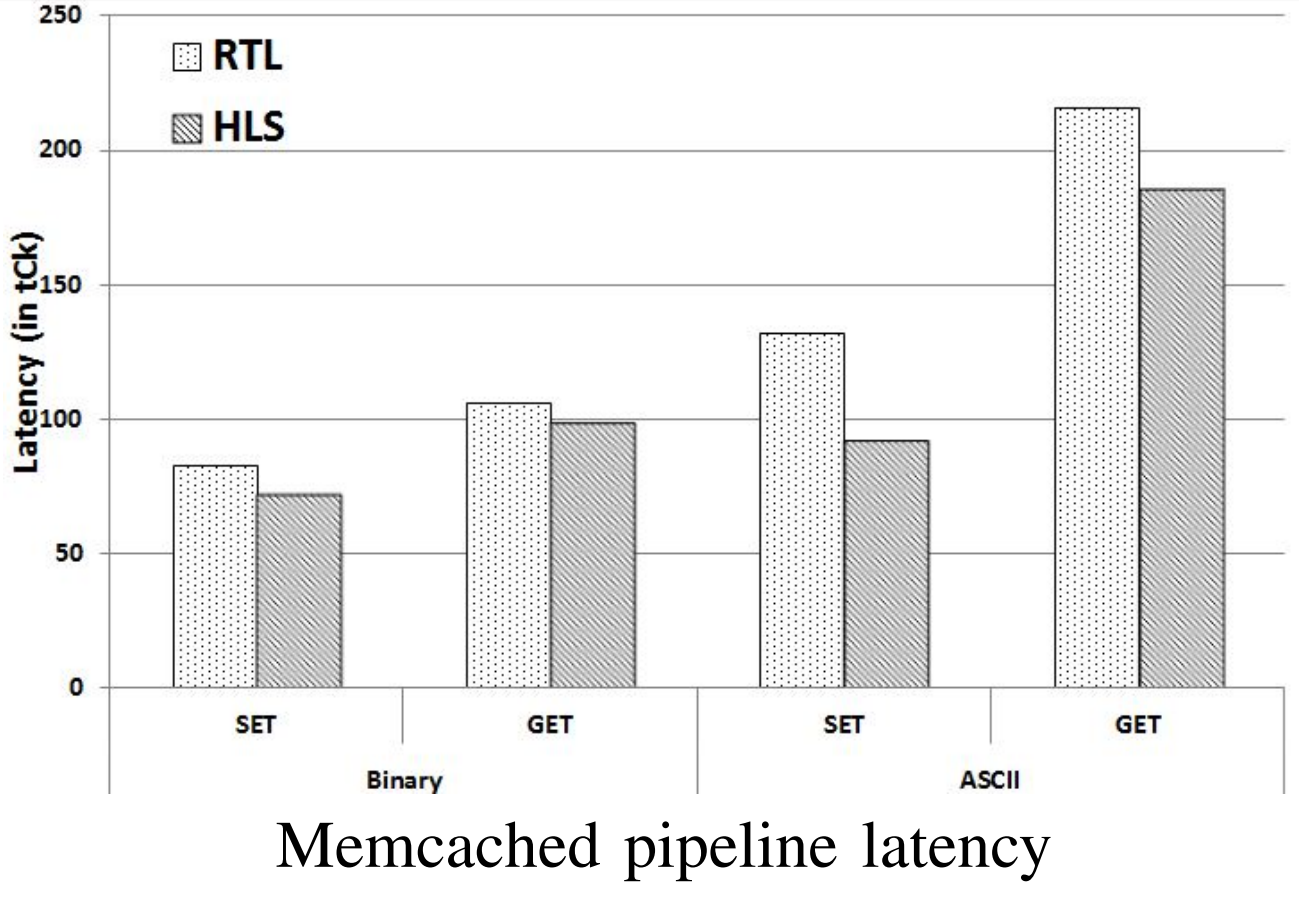
\includegraphics[width=.65\textwidth]{hls_latency}

        \tiny{Image: Karras, Kimon, Michaela Blott, and Kees Vissers.
        "High-Level Synthesis Case Study: Implementation of a Memcached
        Server." arXiv preprint arXiv:1408.5387 (2014).}
    \end{center}
\end{frame}

\begin{frame}
    \frametitle{High-Level Synthesis (HLS) for FPGAs}
    \alert{Qualitatively}, with \alert{less effort}:
    \begin{center}
        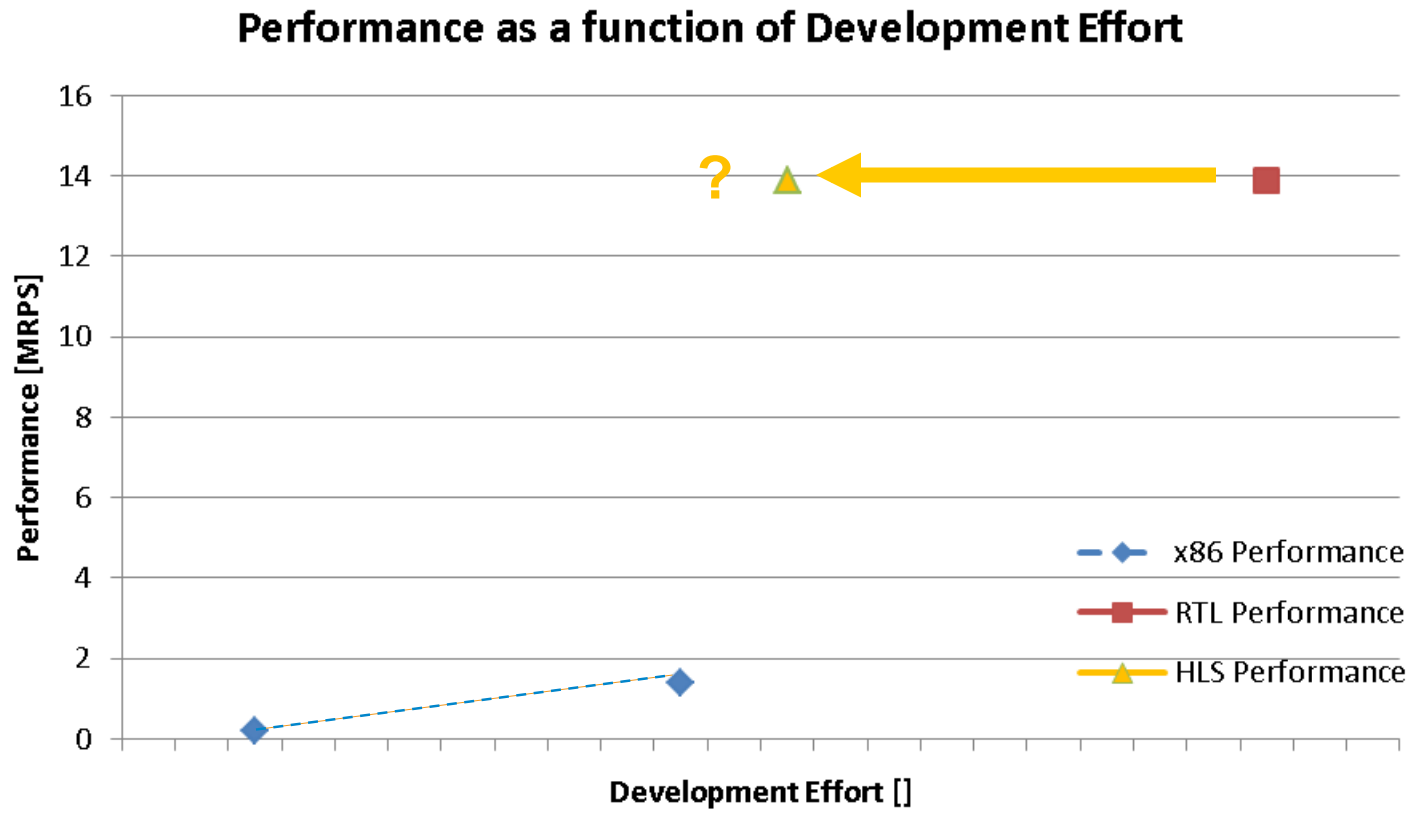
\includegraphics[width=.76\textwidth]{hls_loweffort}

        \tiny{Image: Blott, Michaela, et al. "Achieving 10Gbps line-rate
        key-value stores with FPGAs." Presented as part of the 5th USENIX
        Workshop on Hot Topics in Cloud Computing. 2013.}
    \end{center}
\end{frame}

\begin{frame}
    \frametitle{High-Level Synthesis (HLS) for FPGAs}
    This is an \alert{old issue}:
    \begin{center}
        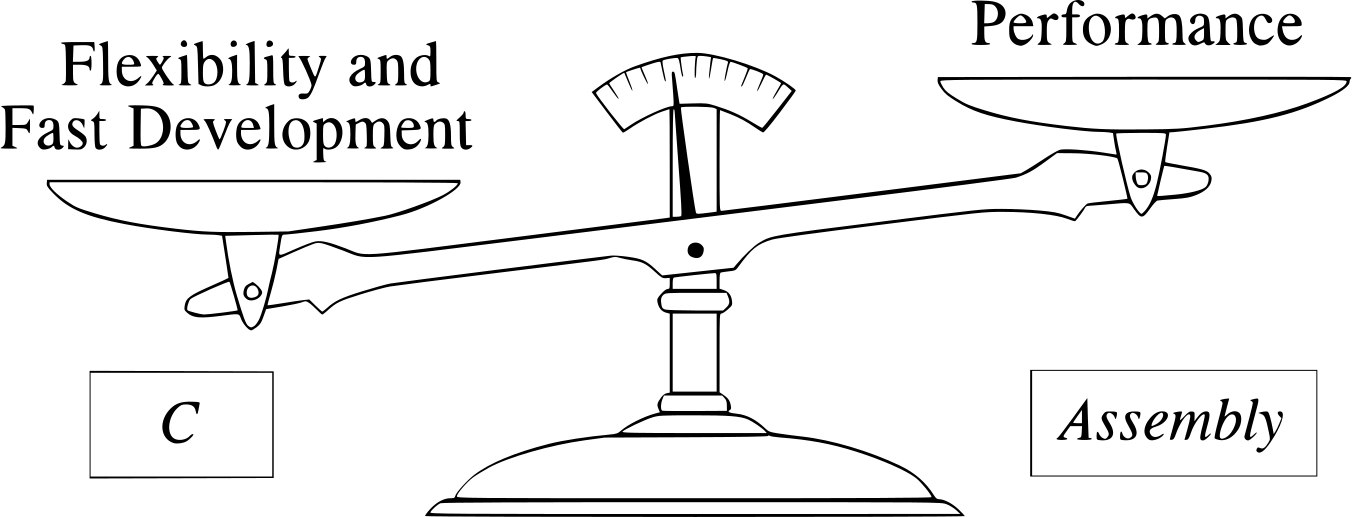
\includegraphics[width=.7\textwidth]{tradeoff_software}

        \tiny{Image: Smith, Steven W. "The scientist and engineer's guide to digital signal processing." 1997}
    \end{center}
\end{frame}

\subsection{Empirical Autotuning}

\begin{frame}
    \frametitle{Empirical Autotuning: Abstract Model}
    \begin{center}
        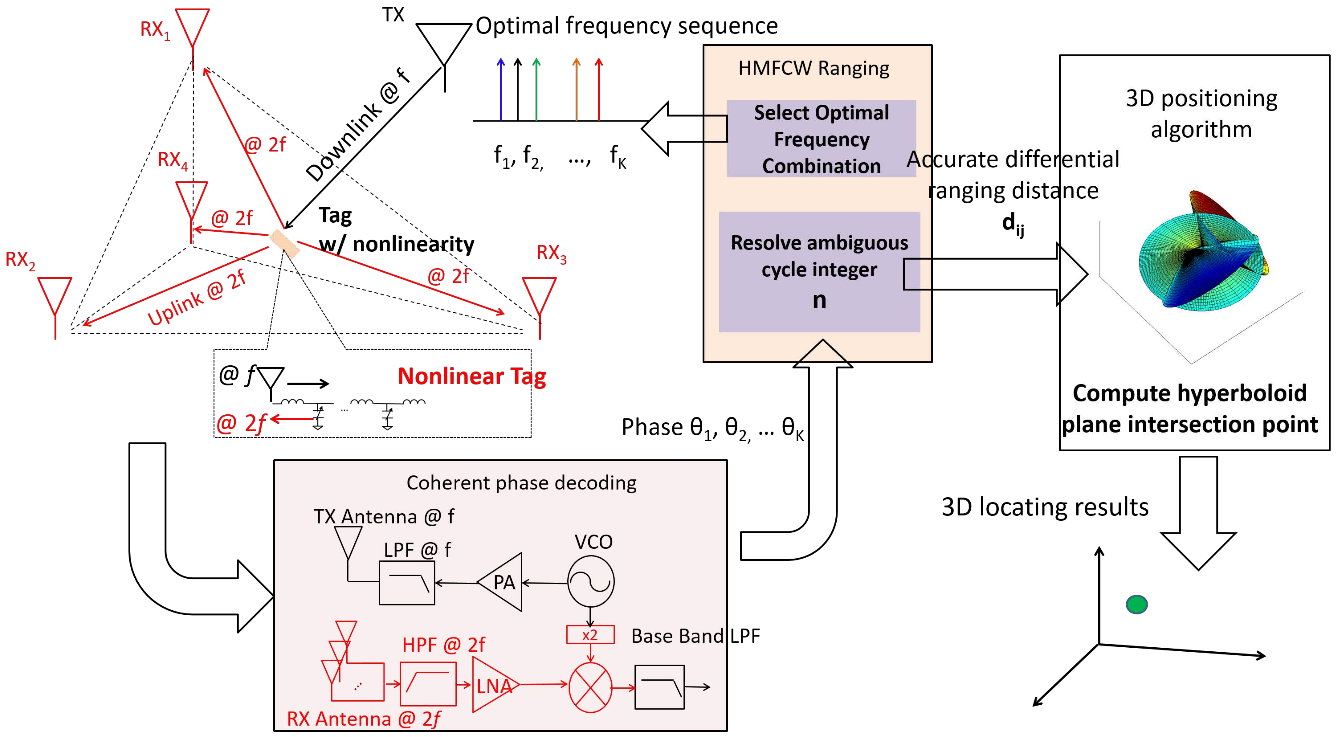
\includegraphics[width=.7\textwidth]{overview}
    \end{center}
\end{frame}

\begin{frame}
    \frametitle{Empirical Autotuning: GPUs}
    \begin{center}
        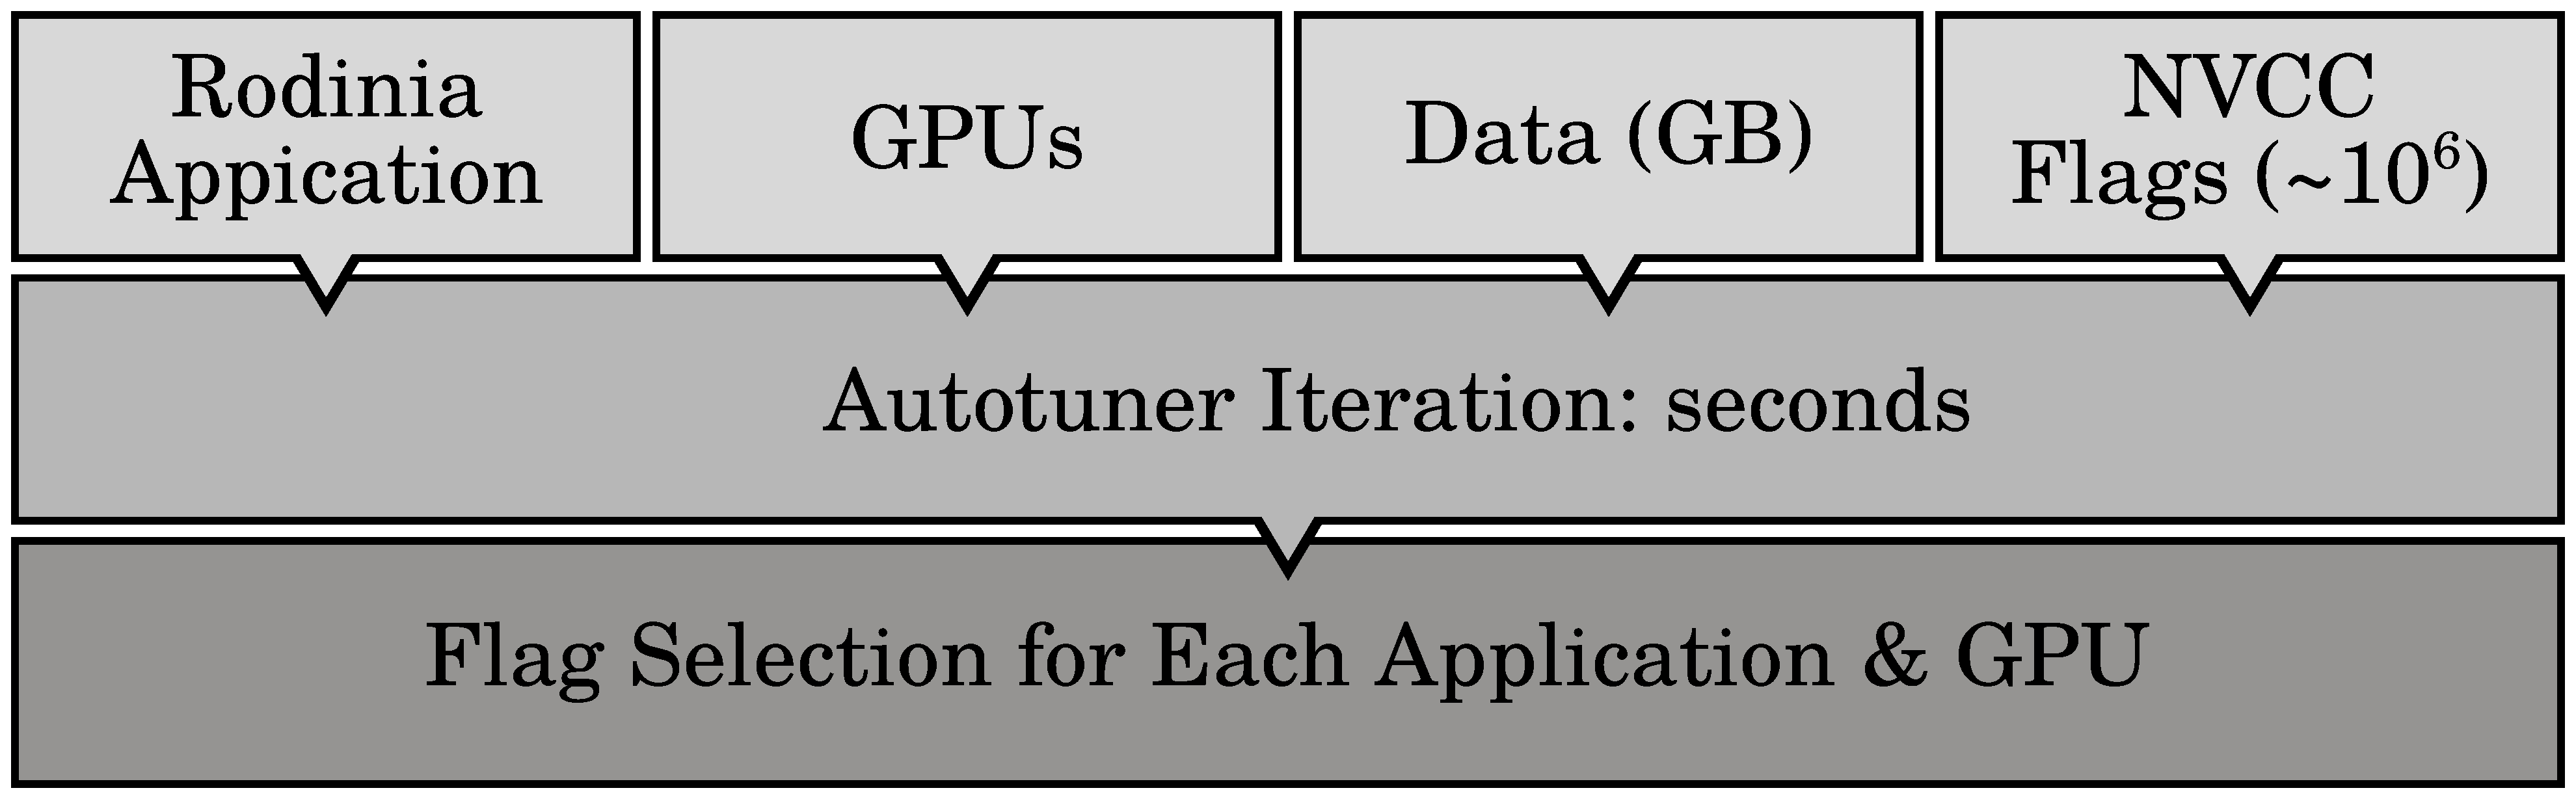
\includegraphics[width=.73\textwidth]{overview_gpus}
    \end{center}

    \begin{itemize}
        \item \alert{1h} of tuning $\rightarrow \; \dfrac{3600s}{\sim{}10^0s} \approx \alert{10^3}$ \alert{iterations}
        \item Up to \alert{$4\times$ speedup}
        \item Paper accepted at Concurrency Computation: Practice and Experience
    \end{itemize}

    \vfill
\end{frame}

\begin{frame}
    \frametitle{Empirical Autotuning: Simple FPGA Applications}
    \begin{center}
        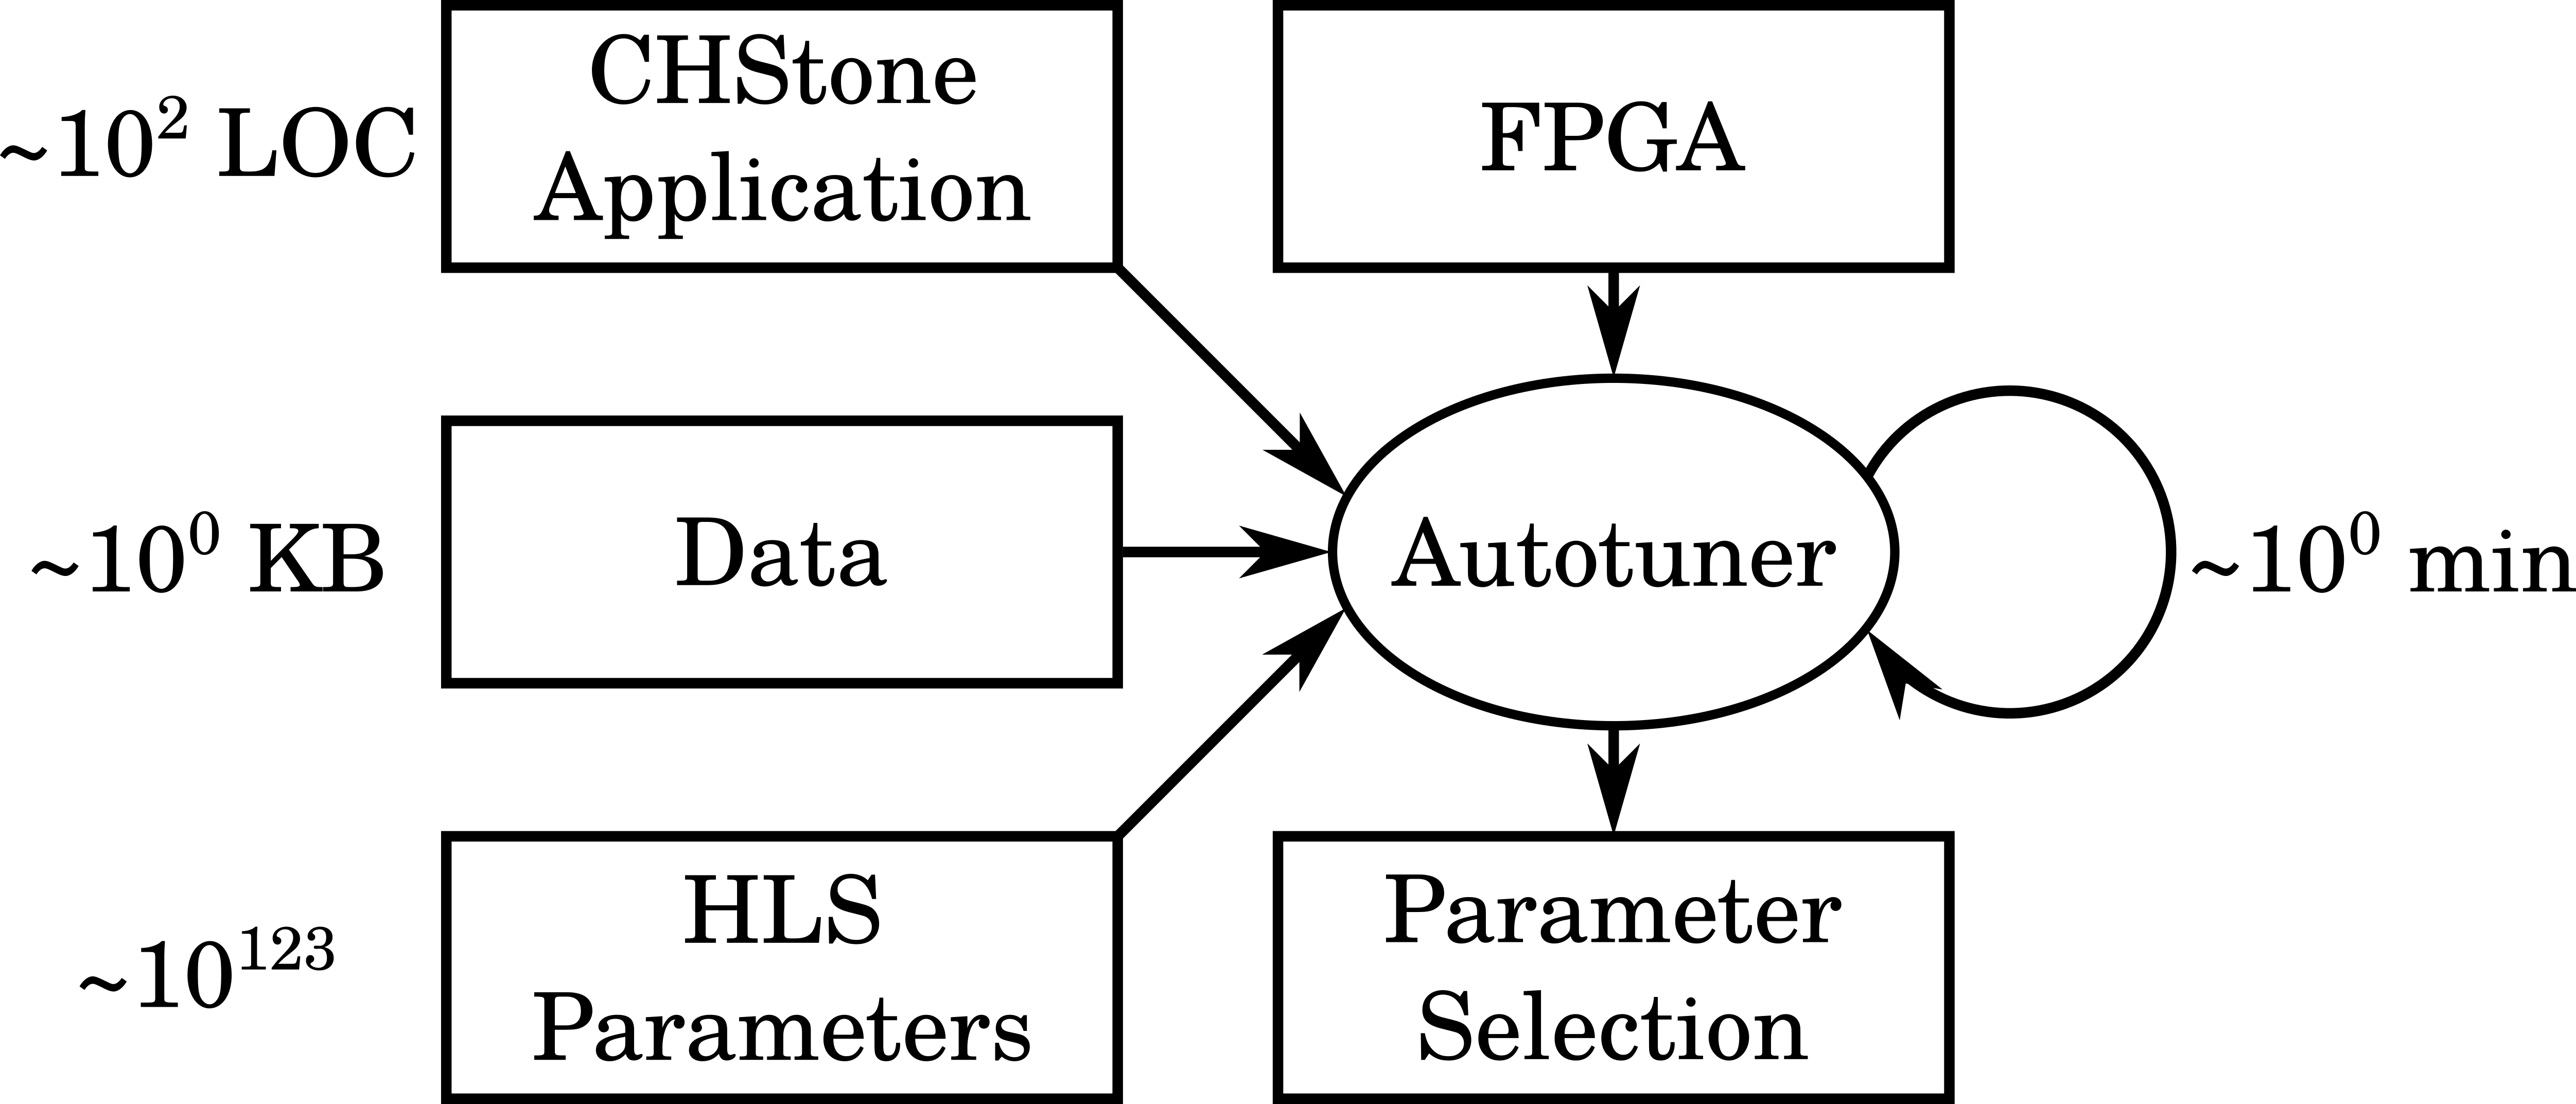
\includegraphics[width=.73\textwidth]{overview_fpgas_small}
    \end{center}

    \begin{itemize}
        \item \alert{1h} of tuning $\rightarrow \; \dfrac{60min}{\sim{}10^0min} \approx \alert{10^1}$ \alert{iterations}
        \item Up to \alert{$2.8\times$ speedup}
    \end{itemize}
\end{frame}

\begin{frame}
    \frametitle{Empirical Autotuning: Complex FPGA Aplications}
    \begin{center}
        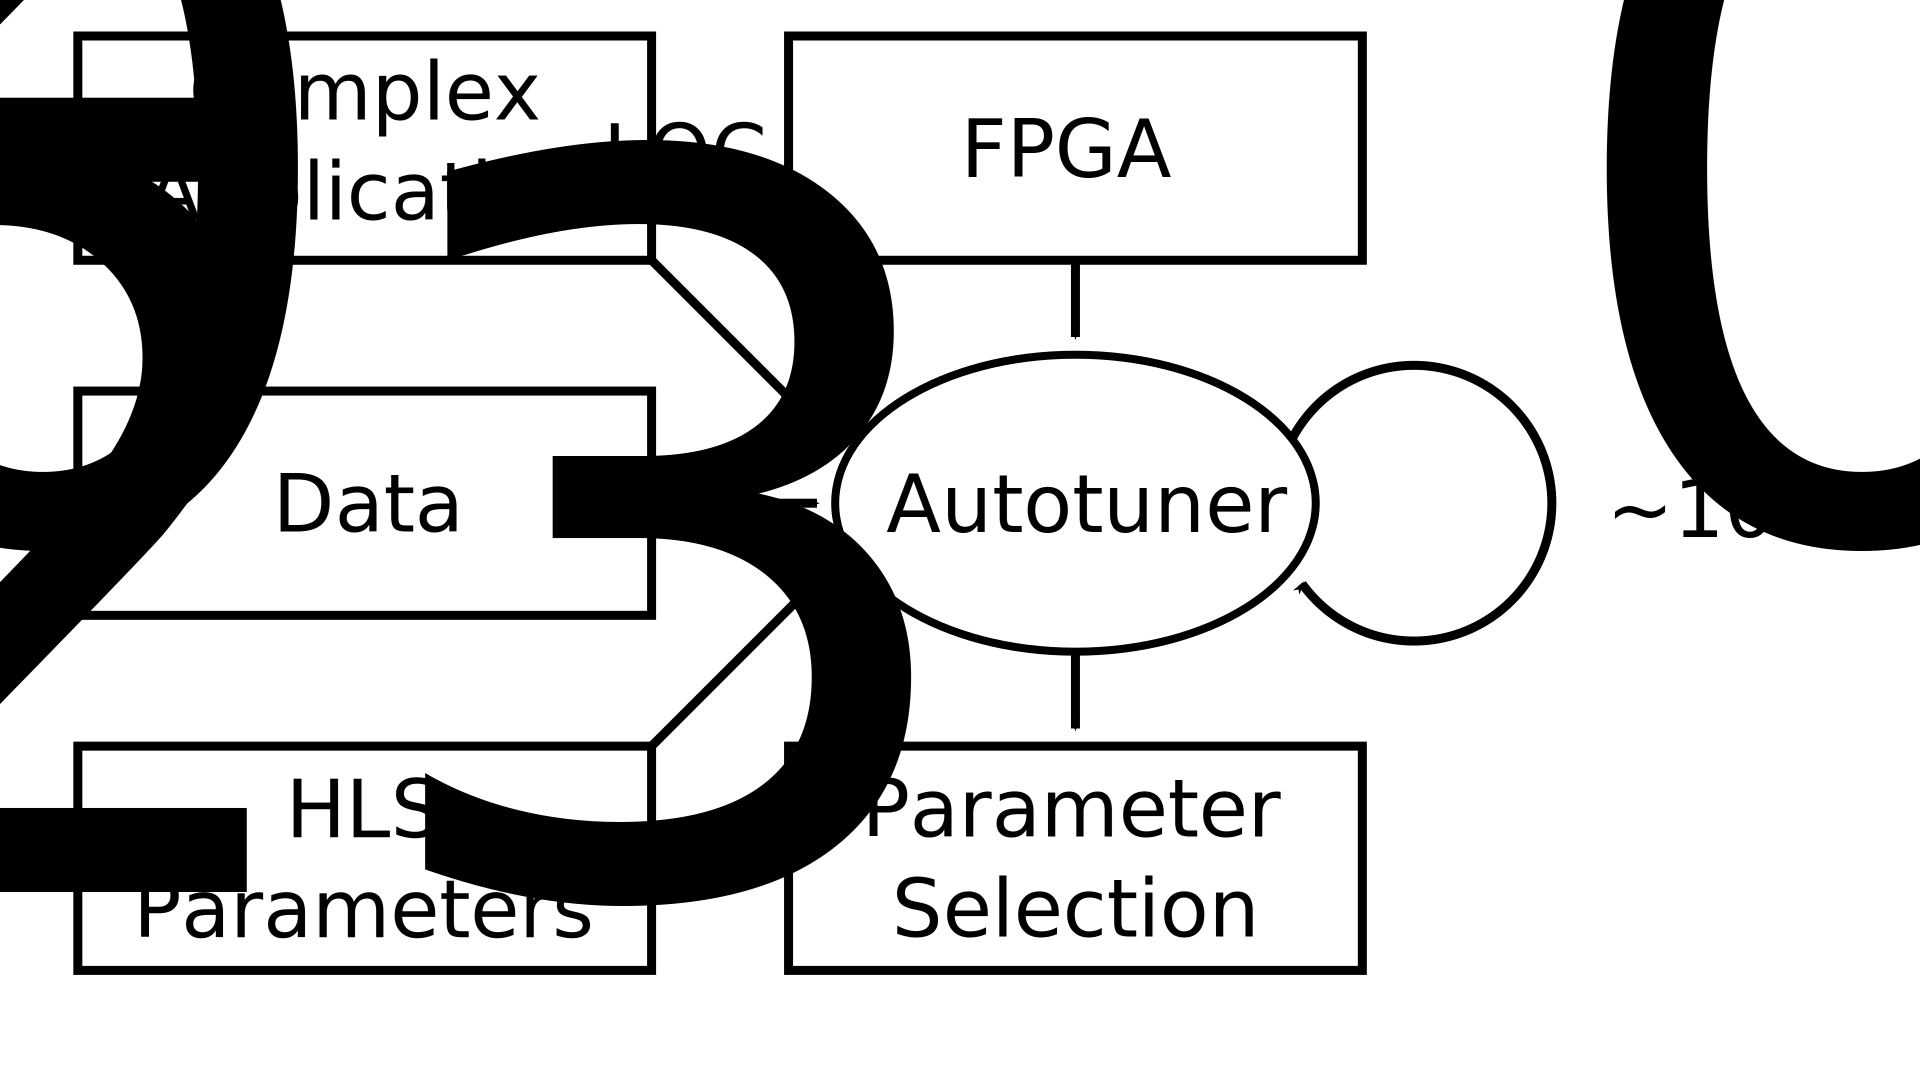
\includegraphics[width=.73\textwidth]{overview_fpgas_big}
    \end{center}

    \begin{itemize}
        \item \alert{1h} of tuning $\rightarrow \; \dfrac{1h}{\sim{}10^0h} \approx \alert{10^0}$ \alert{iterations}
        \item Iterations now \alert{take too long}
    \end{itemize}
\end{frame}

\subsection{Objective}

\begin{frame}
    \frametitle{Autotuning High-Level Synthesis for FPGAs: Objective}
    Given a \alert{sequential program} implemented in a \alert{high-level
    language} and a \alert{hardware accelerator}, our objective is to implement
    an \alert{autotuner} able to determine:

    \begin{itemize}
        \item \alert{Functions that should be offloaded} to the hardware accelerator
        \item \alert{Optimizations} that should be applied to each function
    \end{itemize}
\end{frame}



\section{Autotuning HLS for FPGAs}

\begin{frame}
    \frametitle{Autotuning HLS for FPGAs}
    \vfill
    What we did so far:

    \begin{itemize}
        \item Implemented an \alert{autotuner} for LegUp's \alert{HLS parameters}
        \item Preliminary \alert{experiments} using the CHStone \alert{benchmark}
        \item Preliminary \alert{comparisons} with related work [1]
    \end{itemize}

    Currently:
    \begin{itemize}
        \item \alert{Estimating cost metrics} during HLS
        \item Performing comprehensive experiments
        \item More \alert{complex benchmarks}
    \end{itemize}

    \begin{center}
        \tiny{[1] Huang, Qijing, et al. "The effect of compiler optimizations
        on high-level synthesis-generated hardware." ACM Transactions on
        Reconfigurable Technology and Systems (TRETS) 8.3 (2015): 14.}
    \end{center}
\end{frame}

\begin{frame}
    \frametitle{Autotuning HLS for FPGAs: Overview}
    \begin{center}
        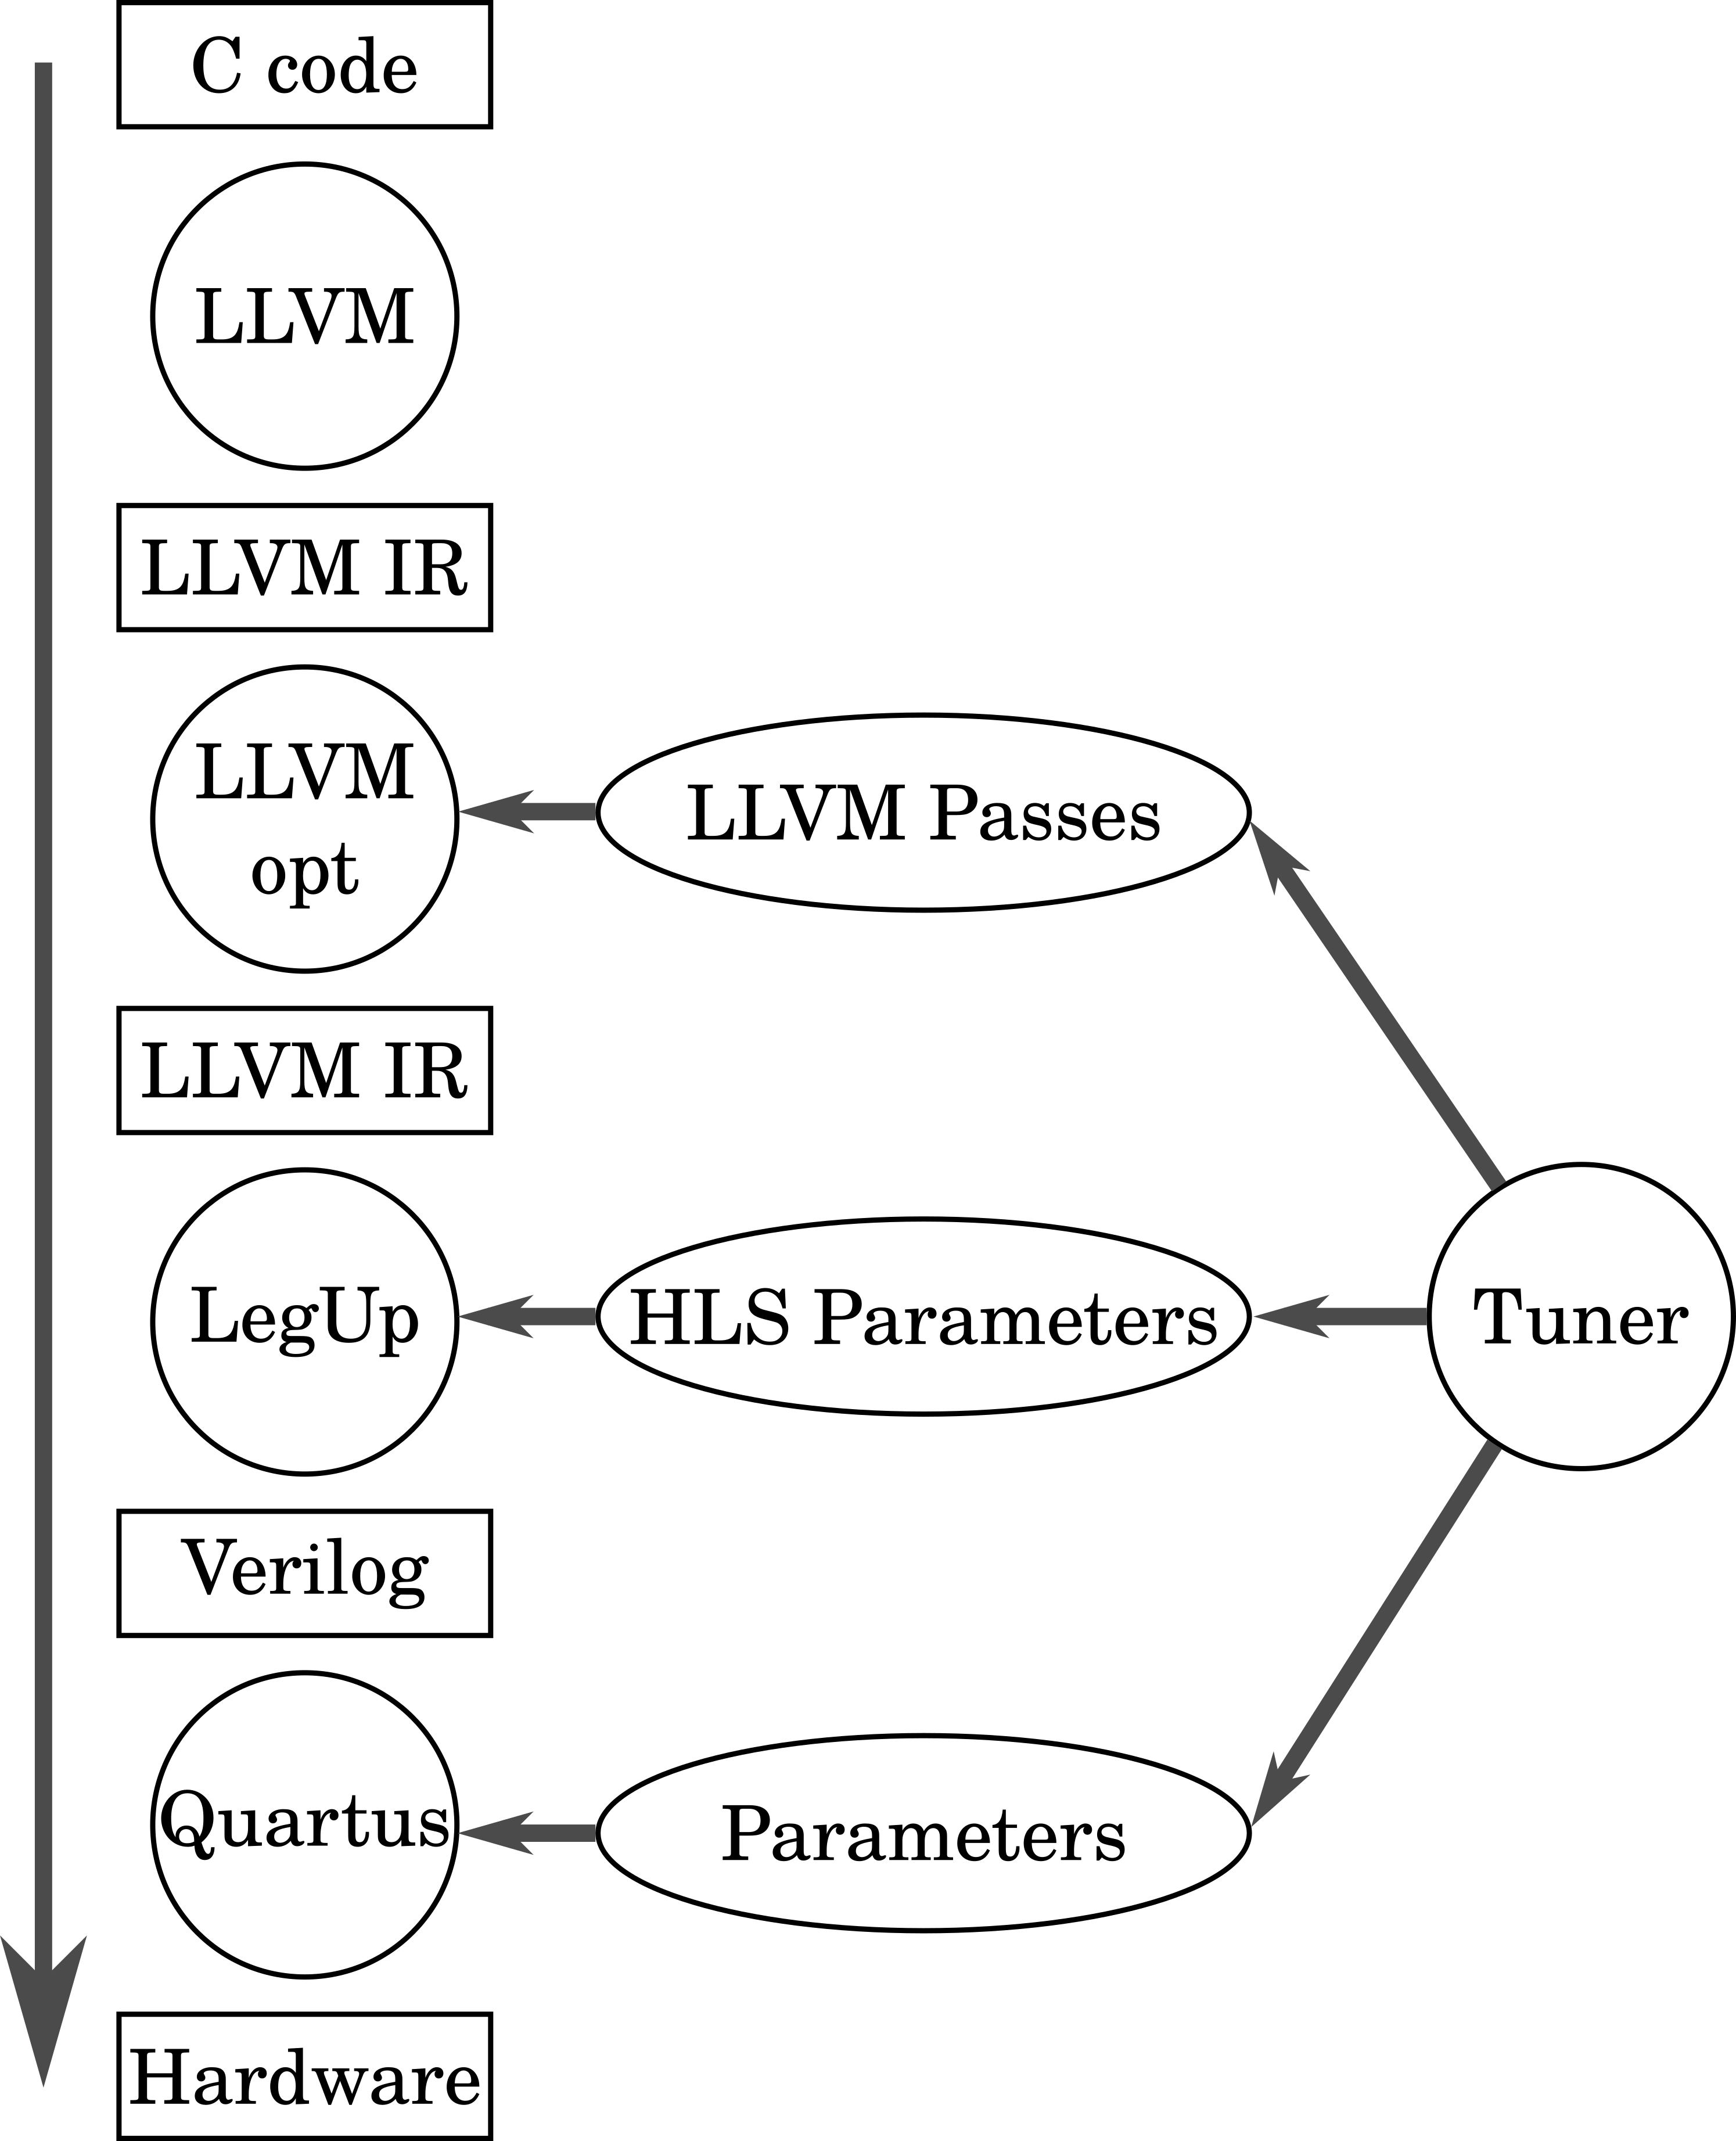
\includegraphics[width=.42\textwidth]{compile_flow_pure}
    \end{center}
\end{frame}

\begin{frame}
    \frametitle{Autotuning HLS for FPGAs: Scope of this Work}
    \begin{center}
        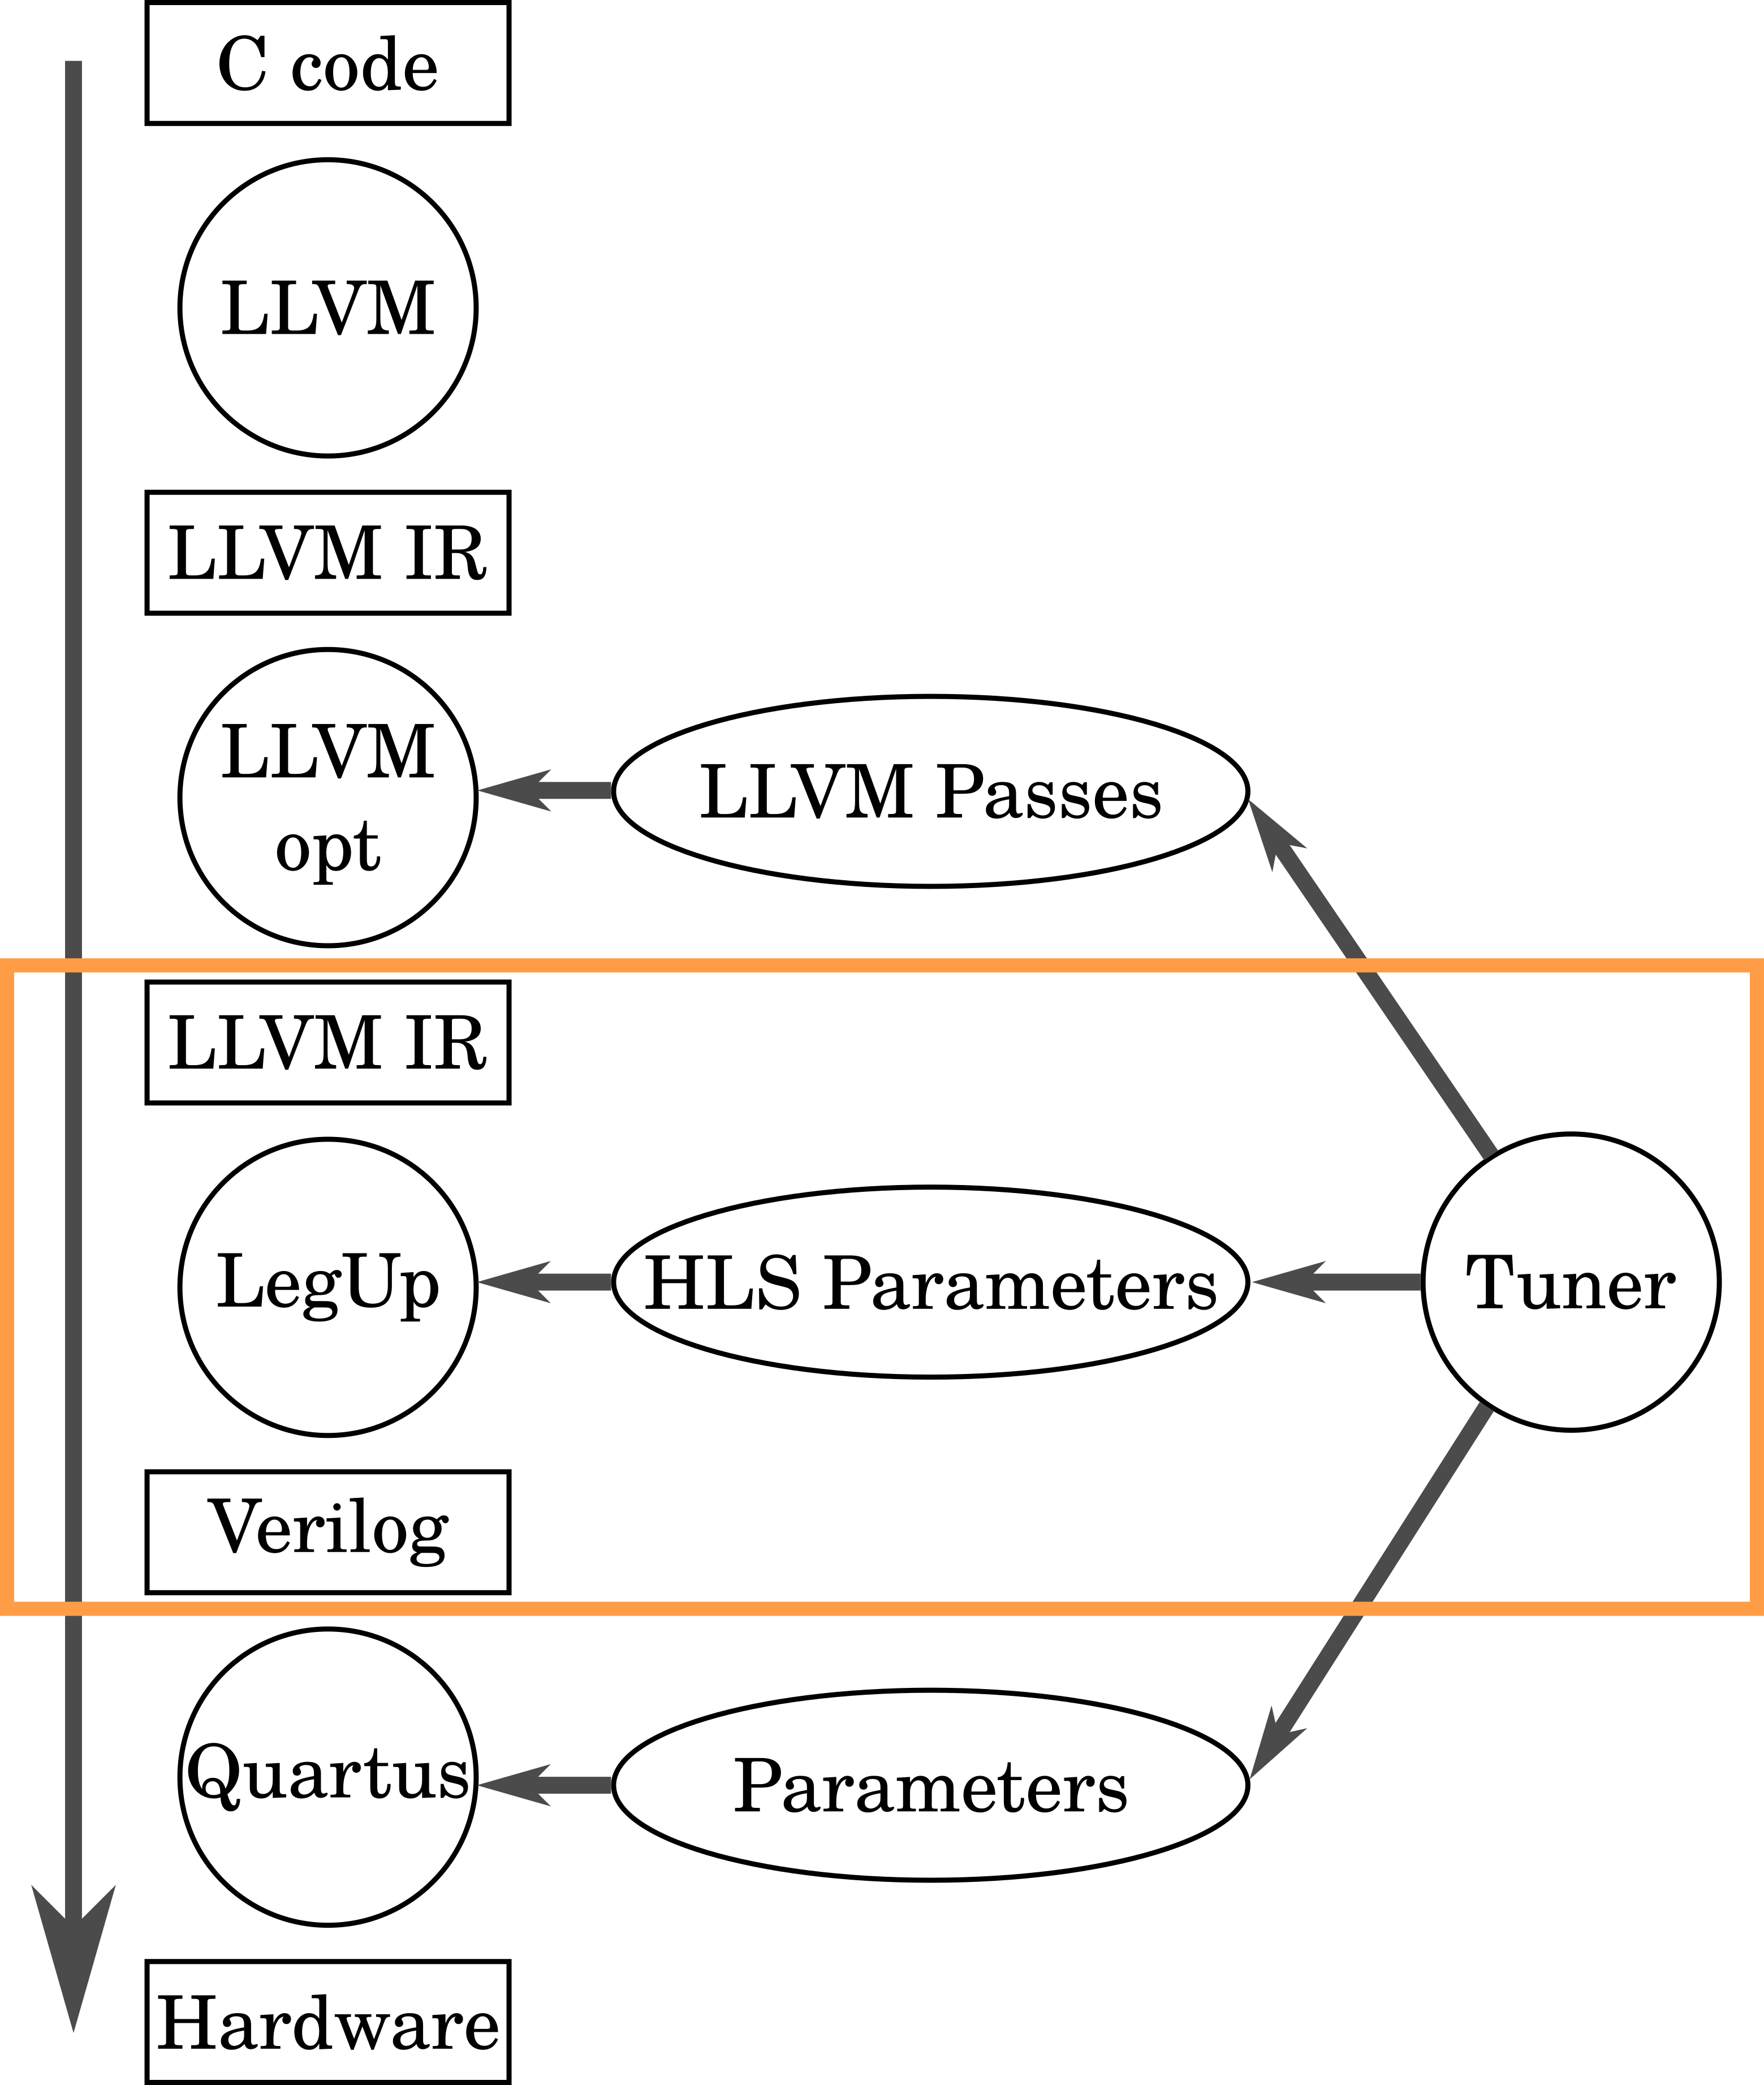
\includegraphics[width=.445\textwidth]{compile_flow_our}
    \end{center}
\end{frame}

\begin{frame}
    \frametitle{Autotuning HLS for FPGAs: Scope of this Work}
    LegUp High-Level Synthesis parameters:
    \begin{itemize}
        \item Constraints that \alert{impact Verilog generation}
        \item Read from a \alert{configuration file}
    \end{itemize}

    Examples:
    \begin{itemize}
        \item \texttt{set\_accelerator\_function}
        \item \texttt{ENABLE\_PATTERN\_SHARING}
    \end{itemize}

    \begin{center}
        \tiny{Source: \url{legup.eecg.utoronto.ca/docs/4.0/constraintsmanual.html\#constraints} [Accessed on 15/09/16]}
    \end{center}
\end{frame}

\begin{frame}
    \frametitle{Autotuning HLS for FPGAs}
    Tools we use:
    \begin{itemize}
        \item OpenTuner: \alert{autotuning framework} in Python
        \item LegUp: LLVM \alert{back-end for Verilog}
        \item Altera Quartus
        \item Docker: \alert{distributed} autotuner execution
        \item CHStone: \alert{HLS benchmark}
    \end{itemize}

    Our code is hosted at GitHub:

    \begin{itemize}
        \item \url{github.com/phrb/legup-dockerfile}
        \item \url{github.com/phrb/legup-tuner}
    \end{itemize}
\end{frame}

\begin{frame}
    \frametitle{Preliminary Results with CHStone: Autotuner Behaviour}
    \begin{center}
        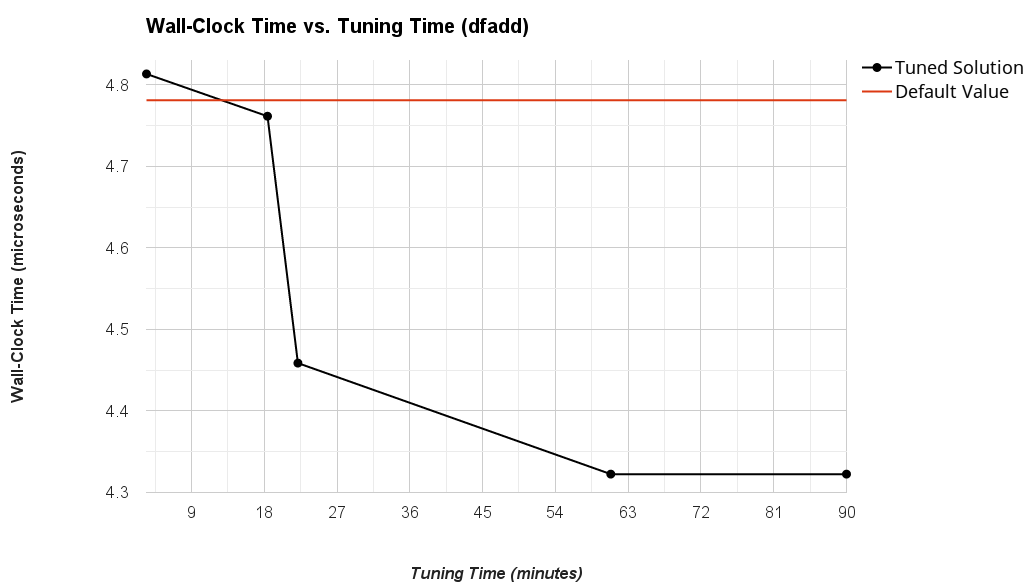
\includegraphics[width=.87\textwidth]{python_dfadd}
    \end{center}
\end{frame}

\begin{frame}
    \frametitle{Preliminary Results: Conclusions}
    After 1h30min of tuning:
    \begin{itemize}
        \item Each configuration took \alert{3 -- 5 min} to compile (CHStone)
        \item Tested \alert{$\sim$30 different configurations}
        \item More complex applications can take \alert{$\sim$10h} to compile
    \end{itemize}

    Our current autotuner \alert{does not scale}:
    \begin{itemize}
        \item Concurrent compilations compete for resources
        \item Python parallelism
    \end{itemize}

    Improving autotuner performance:
    \begin{itemize}
        \item \alert{Estimate cost metrics} during HLS
        \item \alert{Distributed and parallel} autotuning
    \end{itemize}
\end{frame}

\begin{frame}
    \frametitle{The Need for a Cost Model}
    \begin{center}
        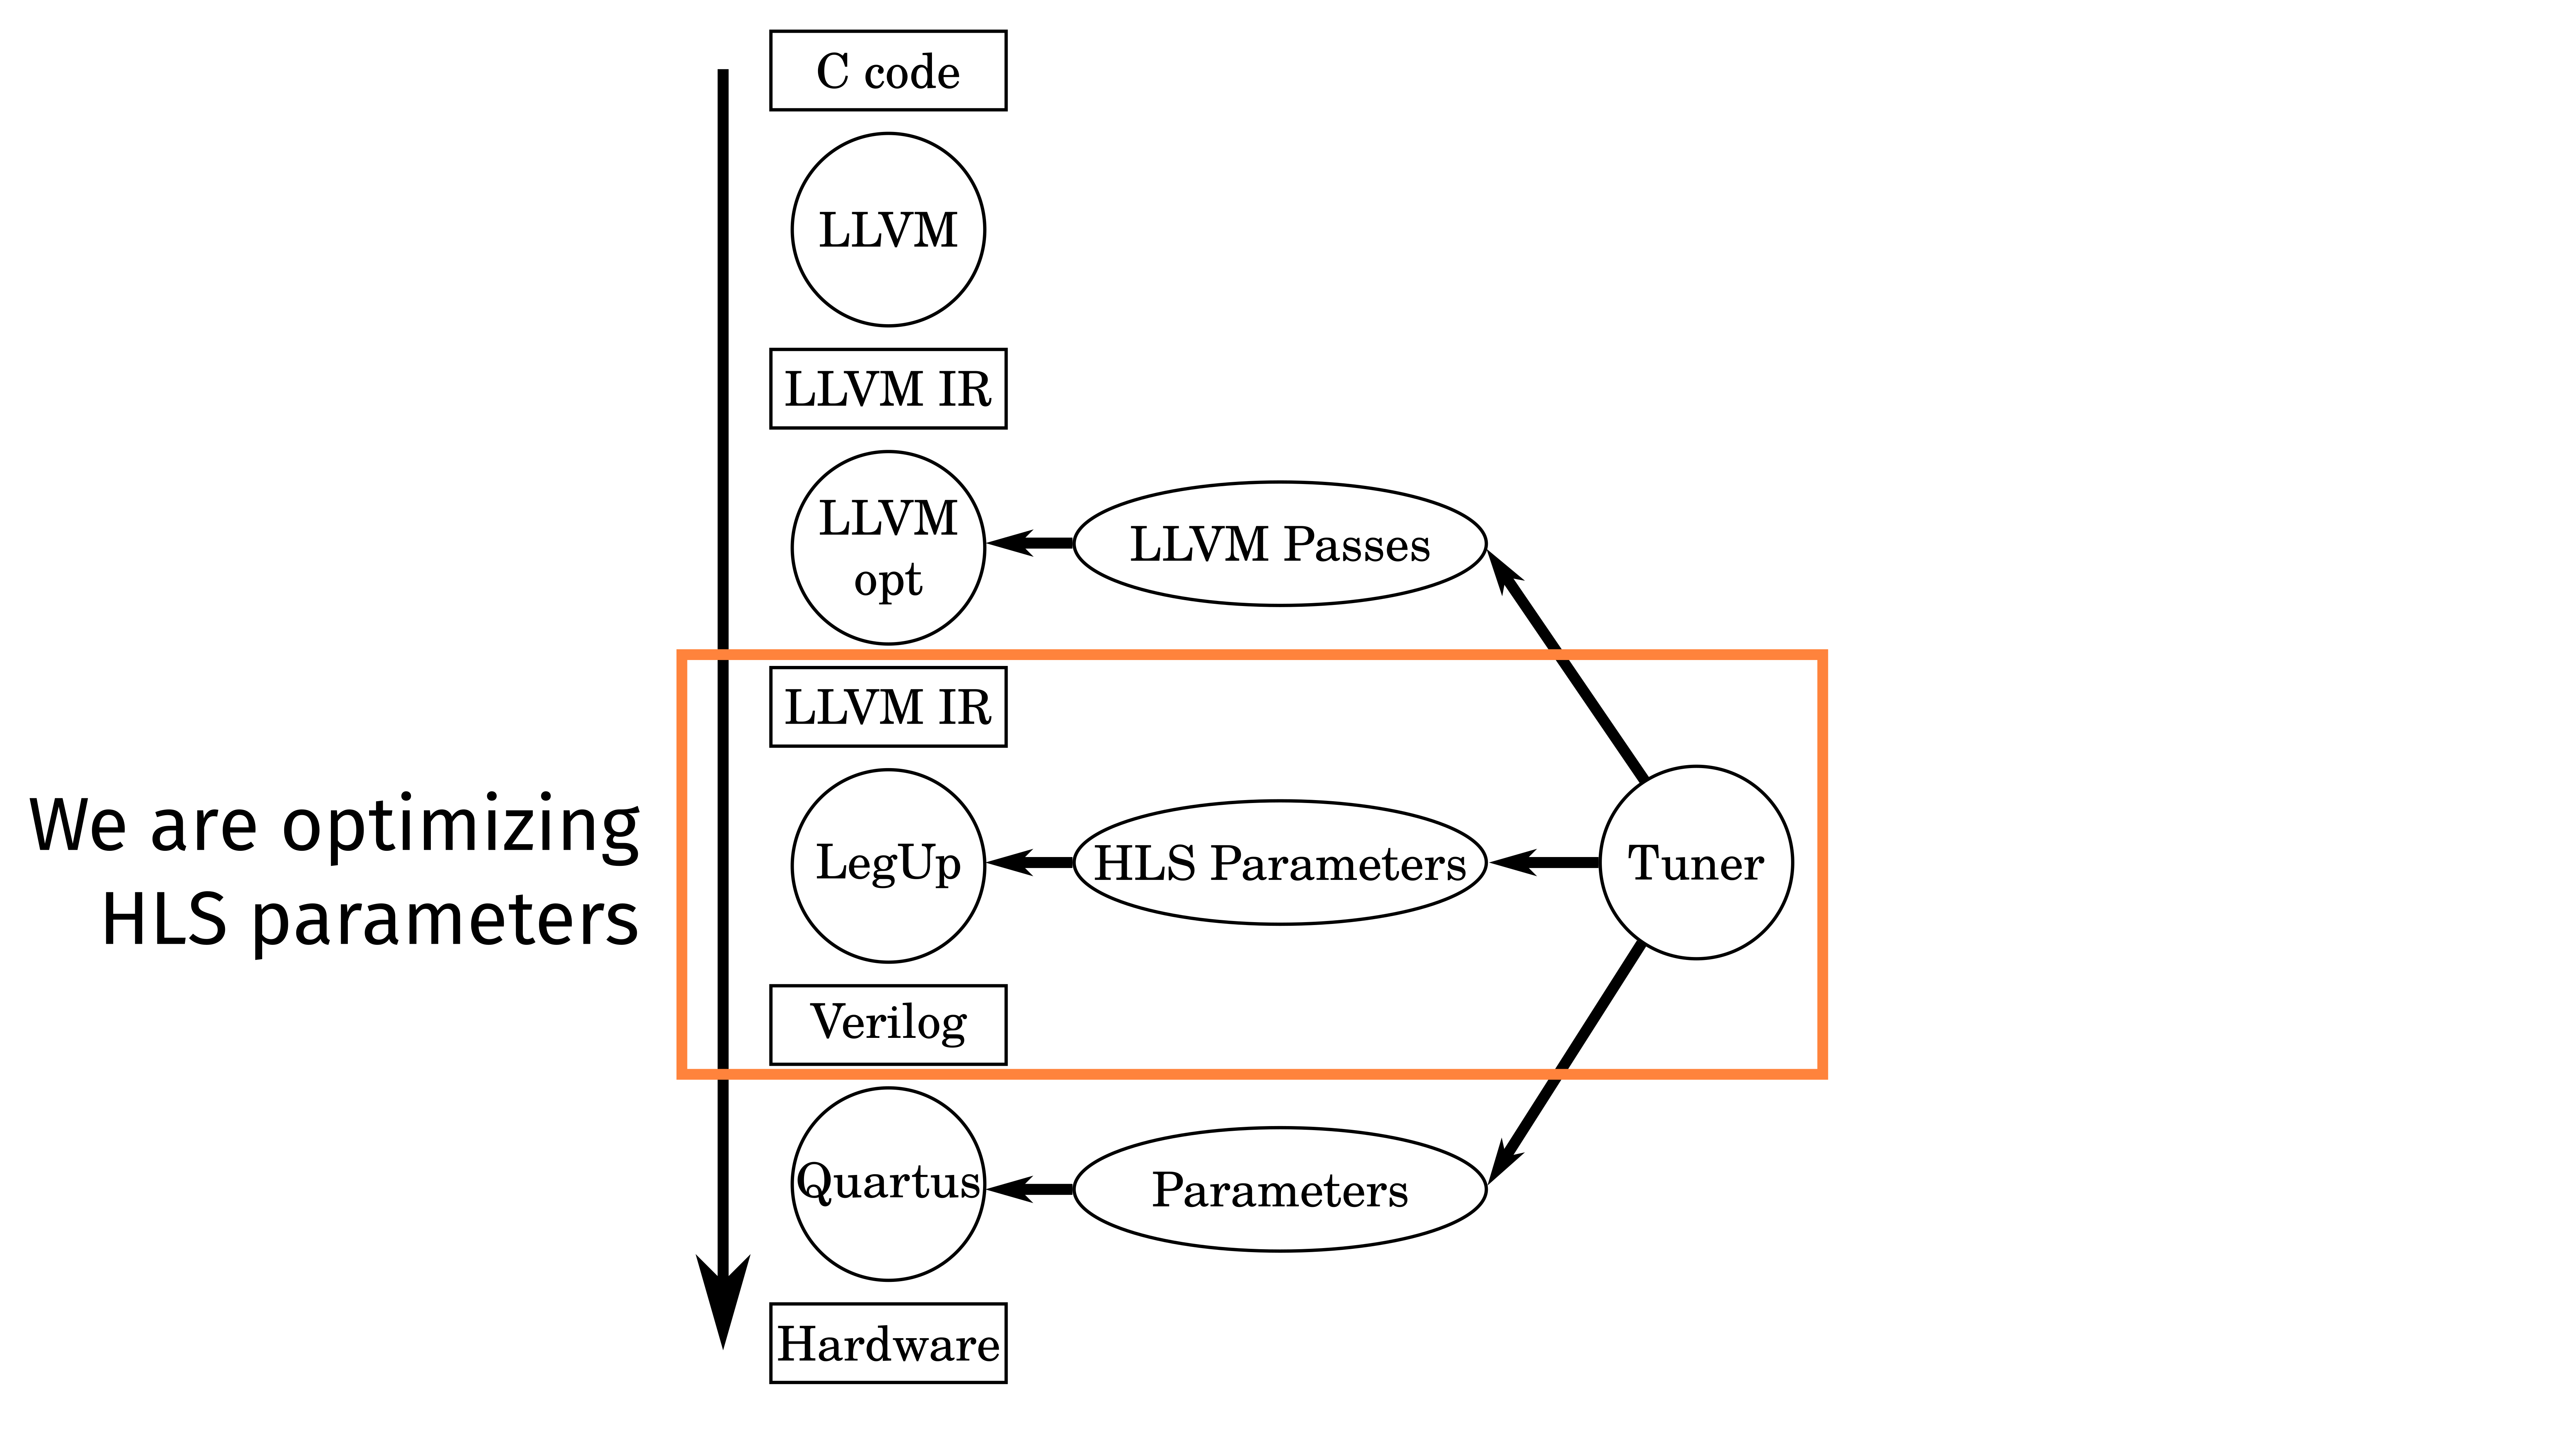
\includegraphics[width=.95\textwidth]{compile_flow_bottleneck_0}
    \end{center}
\end{frame}

\begin{frame}
    \frametitle{The Need for a Cost Model}
    \begin{center}
        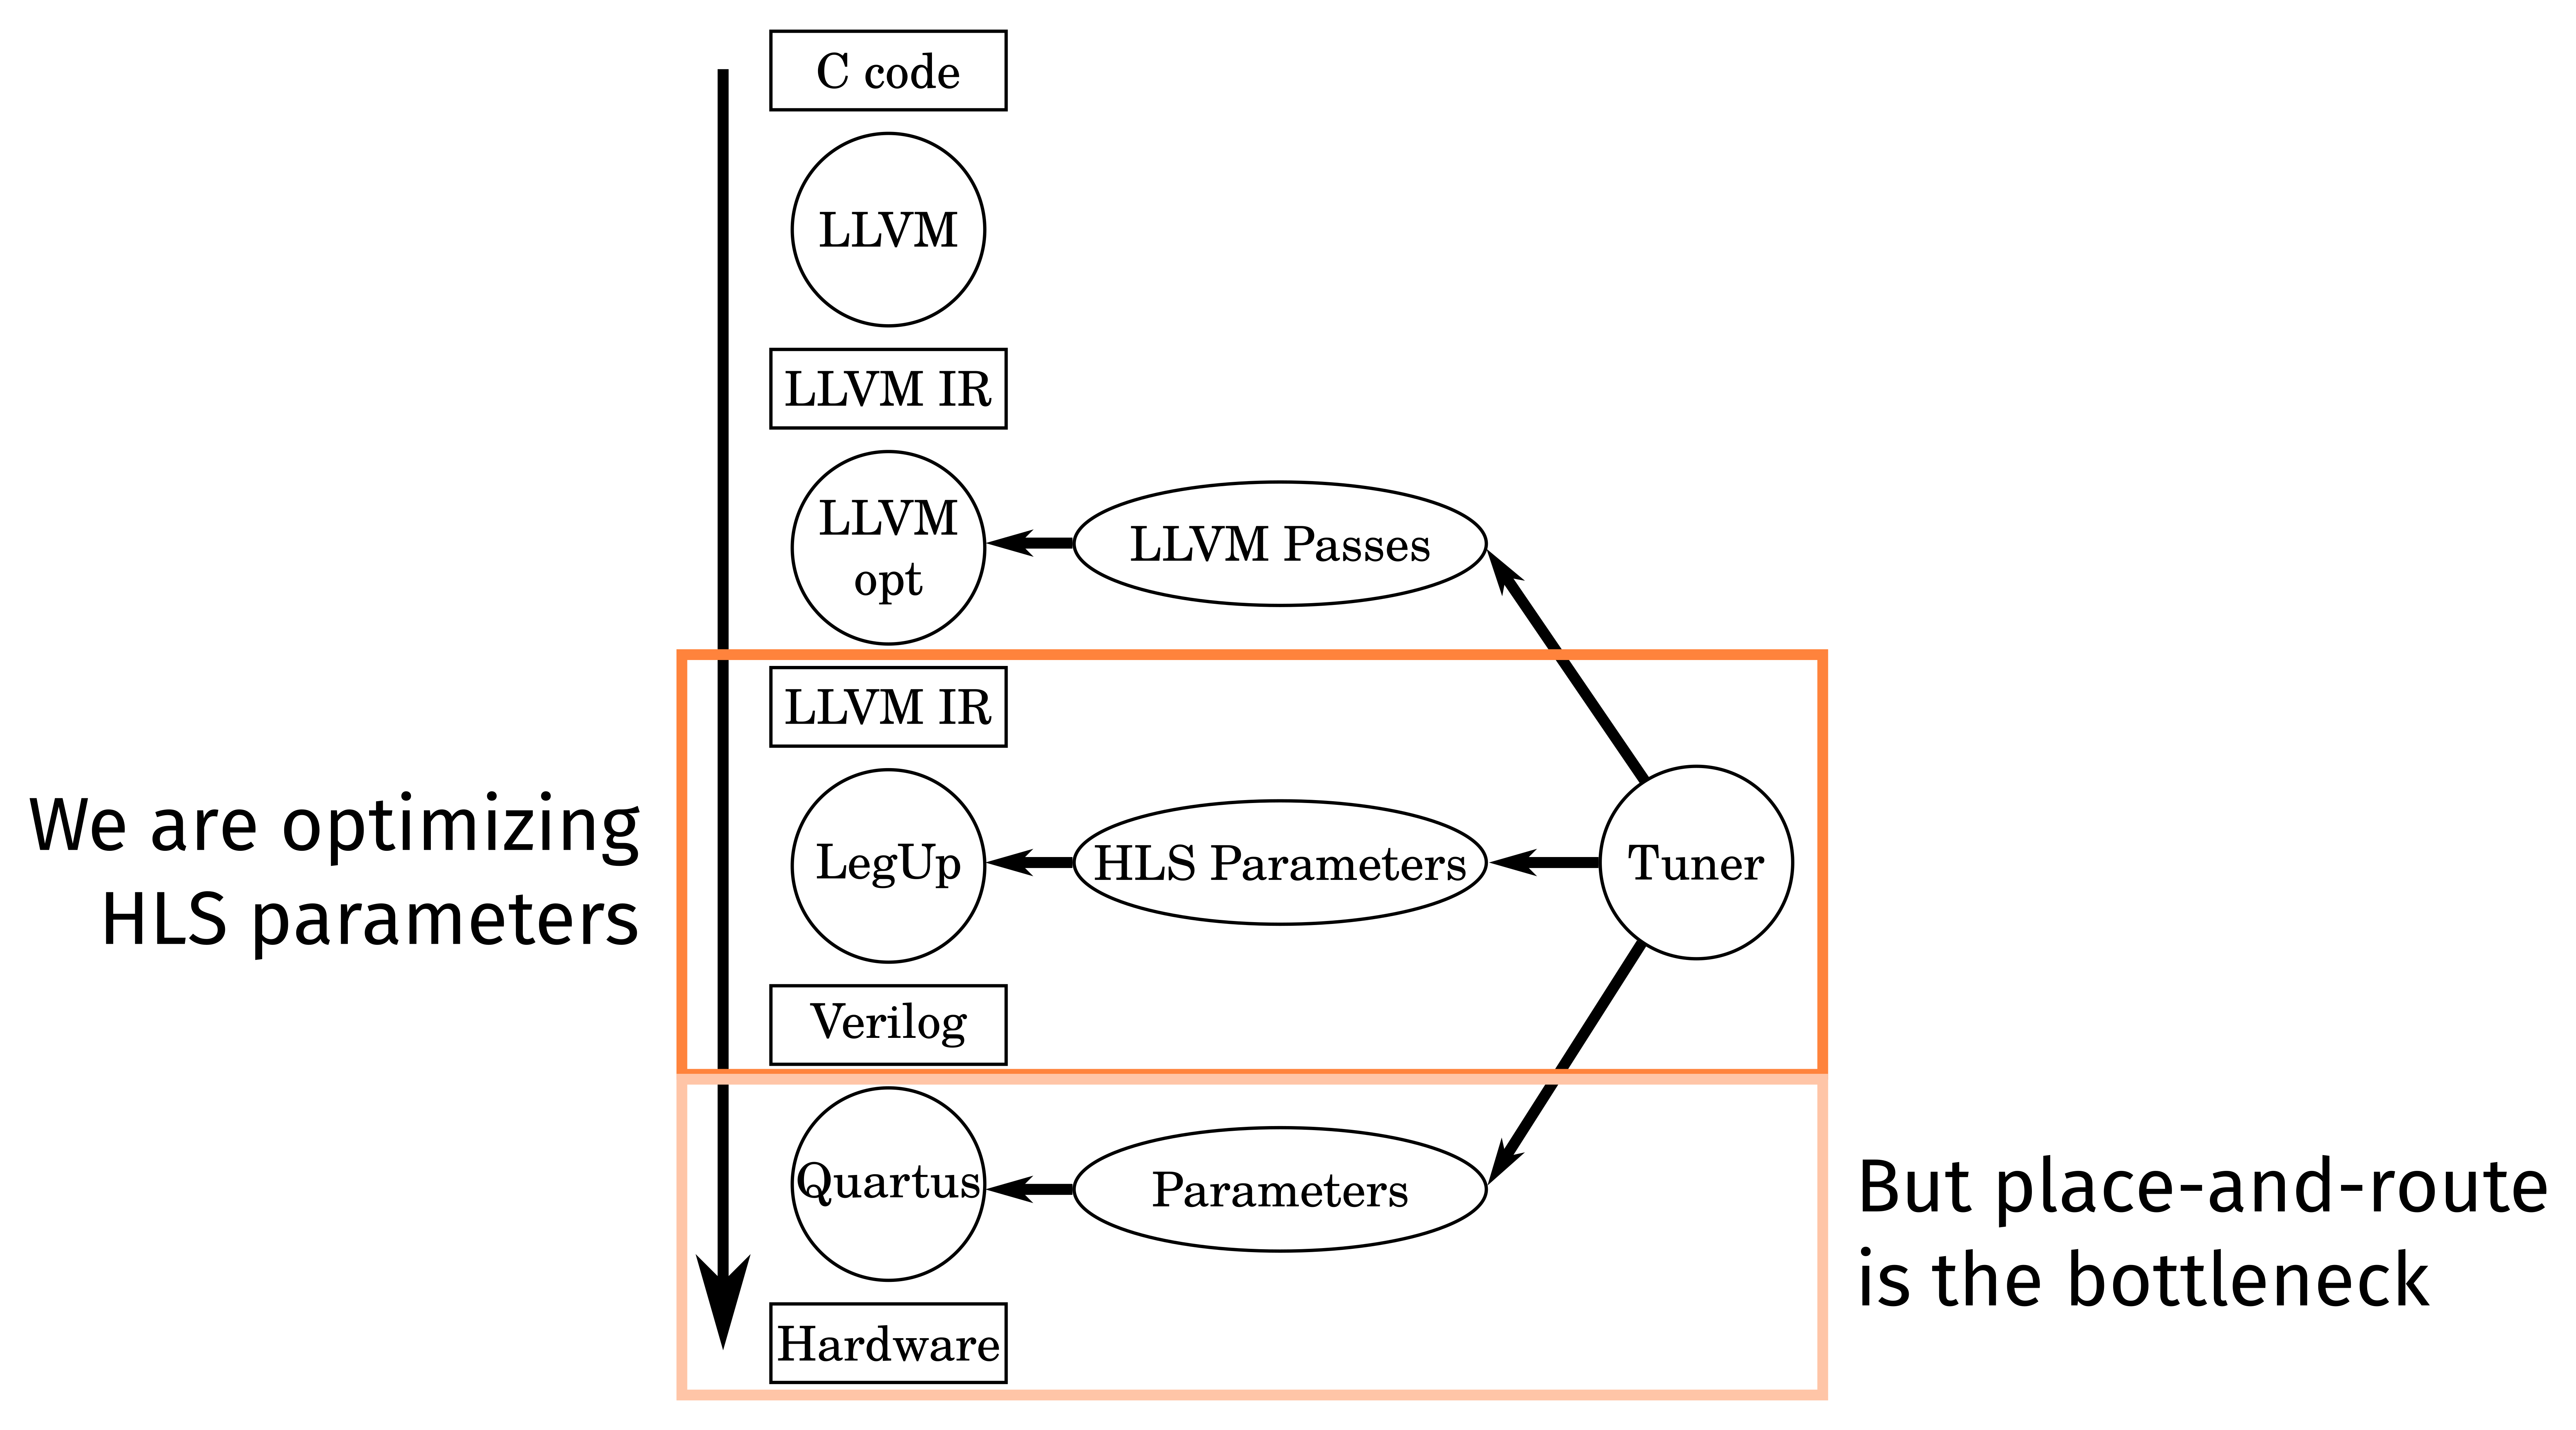
\includegraphics[width=.95\textwidth]{compile_flow_bottleneck_1}
    \end{center}
\end{frame}

\begin{frame}
    \frametitle{The Need for a Cost Model: Complex FPGA Aplications}
    \begin{center}
        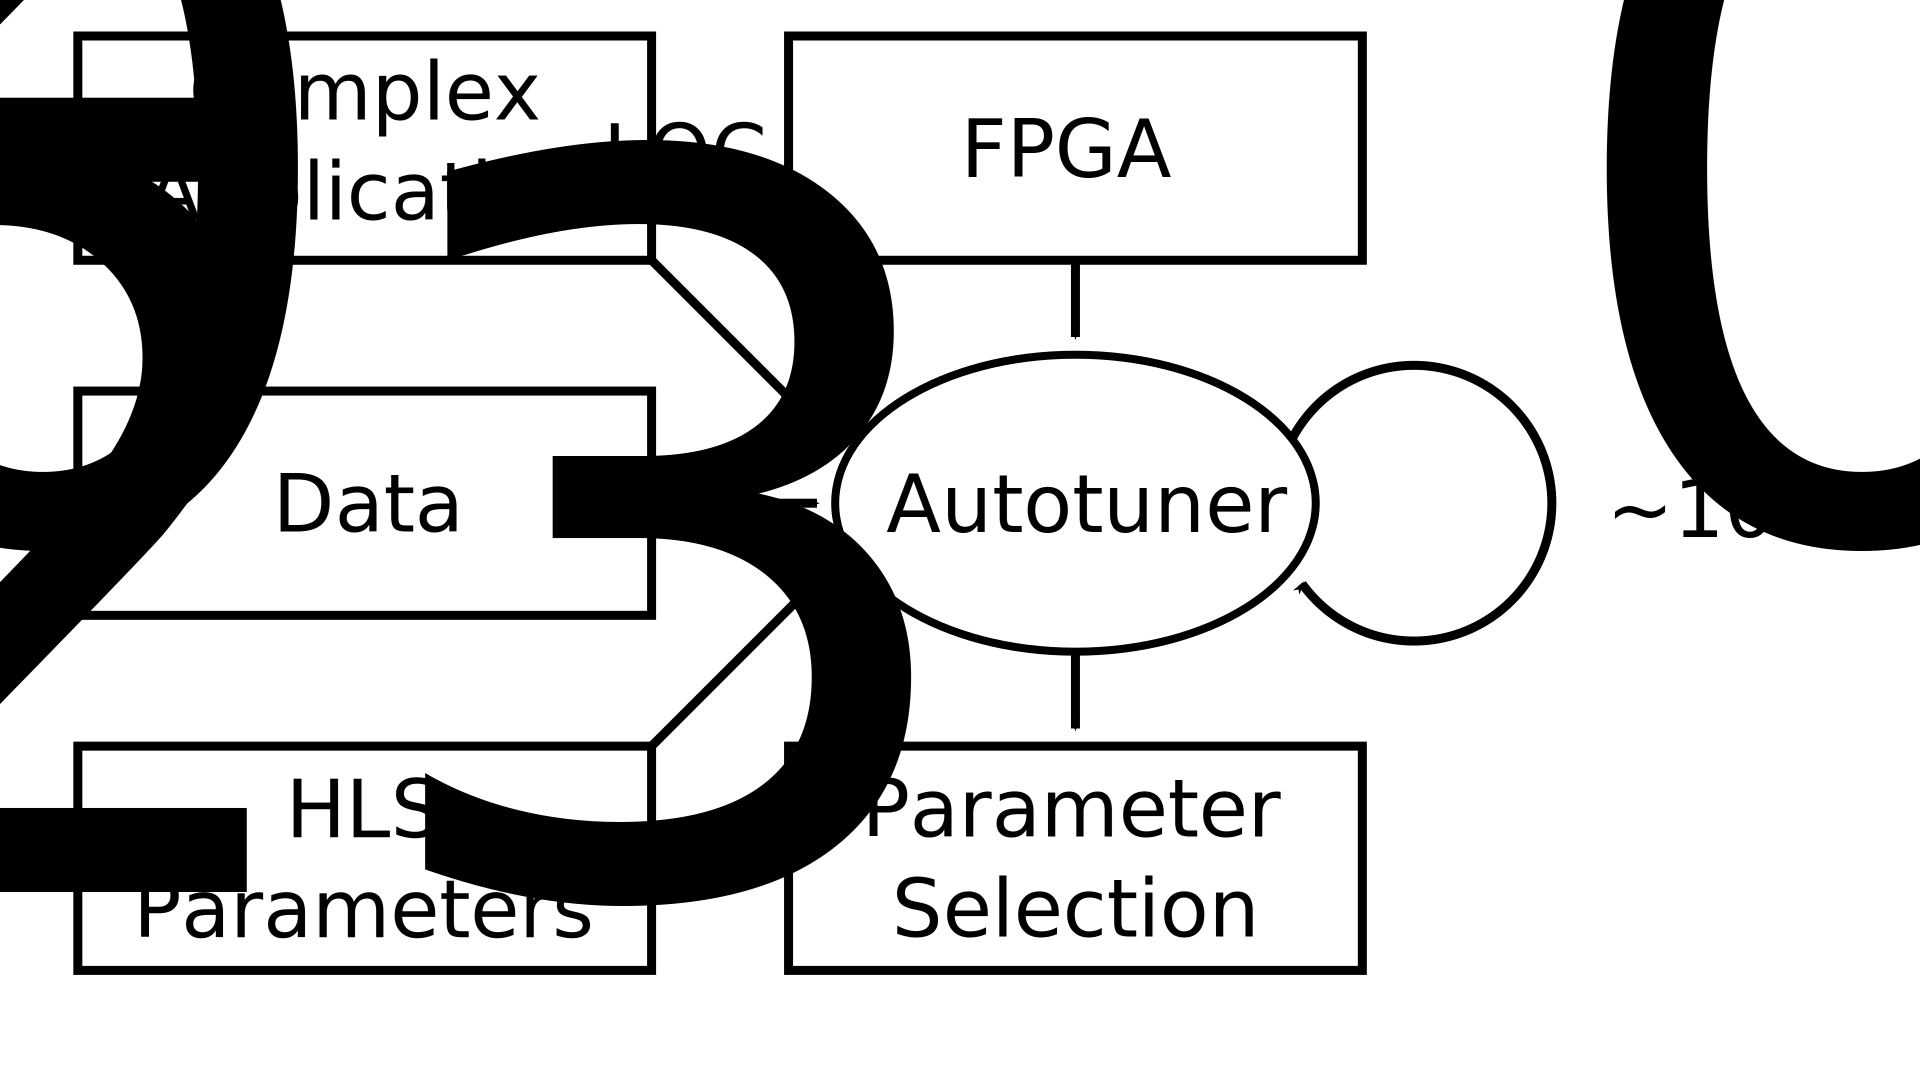
\includegraphics[width=.7\textwidth]{overview_fpgas_big}

        \vfill

        \alert{1h} of tuning $\rightarrow \; \dfrac{1h}{\sim{}10^0h} \approx \alert{10^0}$ \alert{iterations}
    \end{center}
\end{frame}

\begin{frame}
    \frametitle{Huang \textit{et al.}'s work}
        Huang, Qijing, et al. "The effect of compiler optimizations
        on high-level synthesis-generated hardware." ACM Transactions on
        Reconfigurable Technology and Systems (2015):
    \begin{itemize}
        \item Selects \alert{LLVM passes}: optimizations and ordering
        \item Uses \alert{LegUp} as an HLS tool
        \item Targets the Cyclone II device family
        \item Uses the \alert{CHStone benchmark}
        \item Performs \alert{Exhaustive Search}
    \end{itemize}
\end{frame}

\begin{frame}
    \frametitle{Huang \textit{et al.}'s work: Scope}
    \begin{center}
        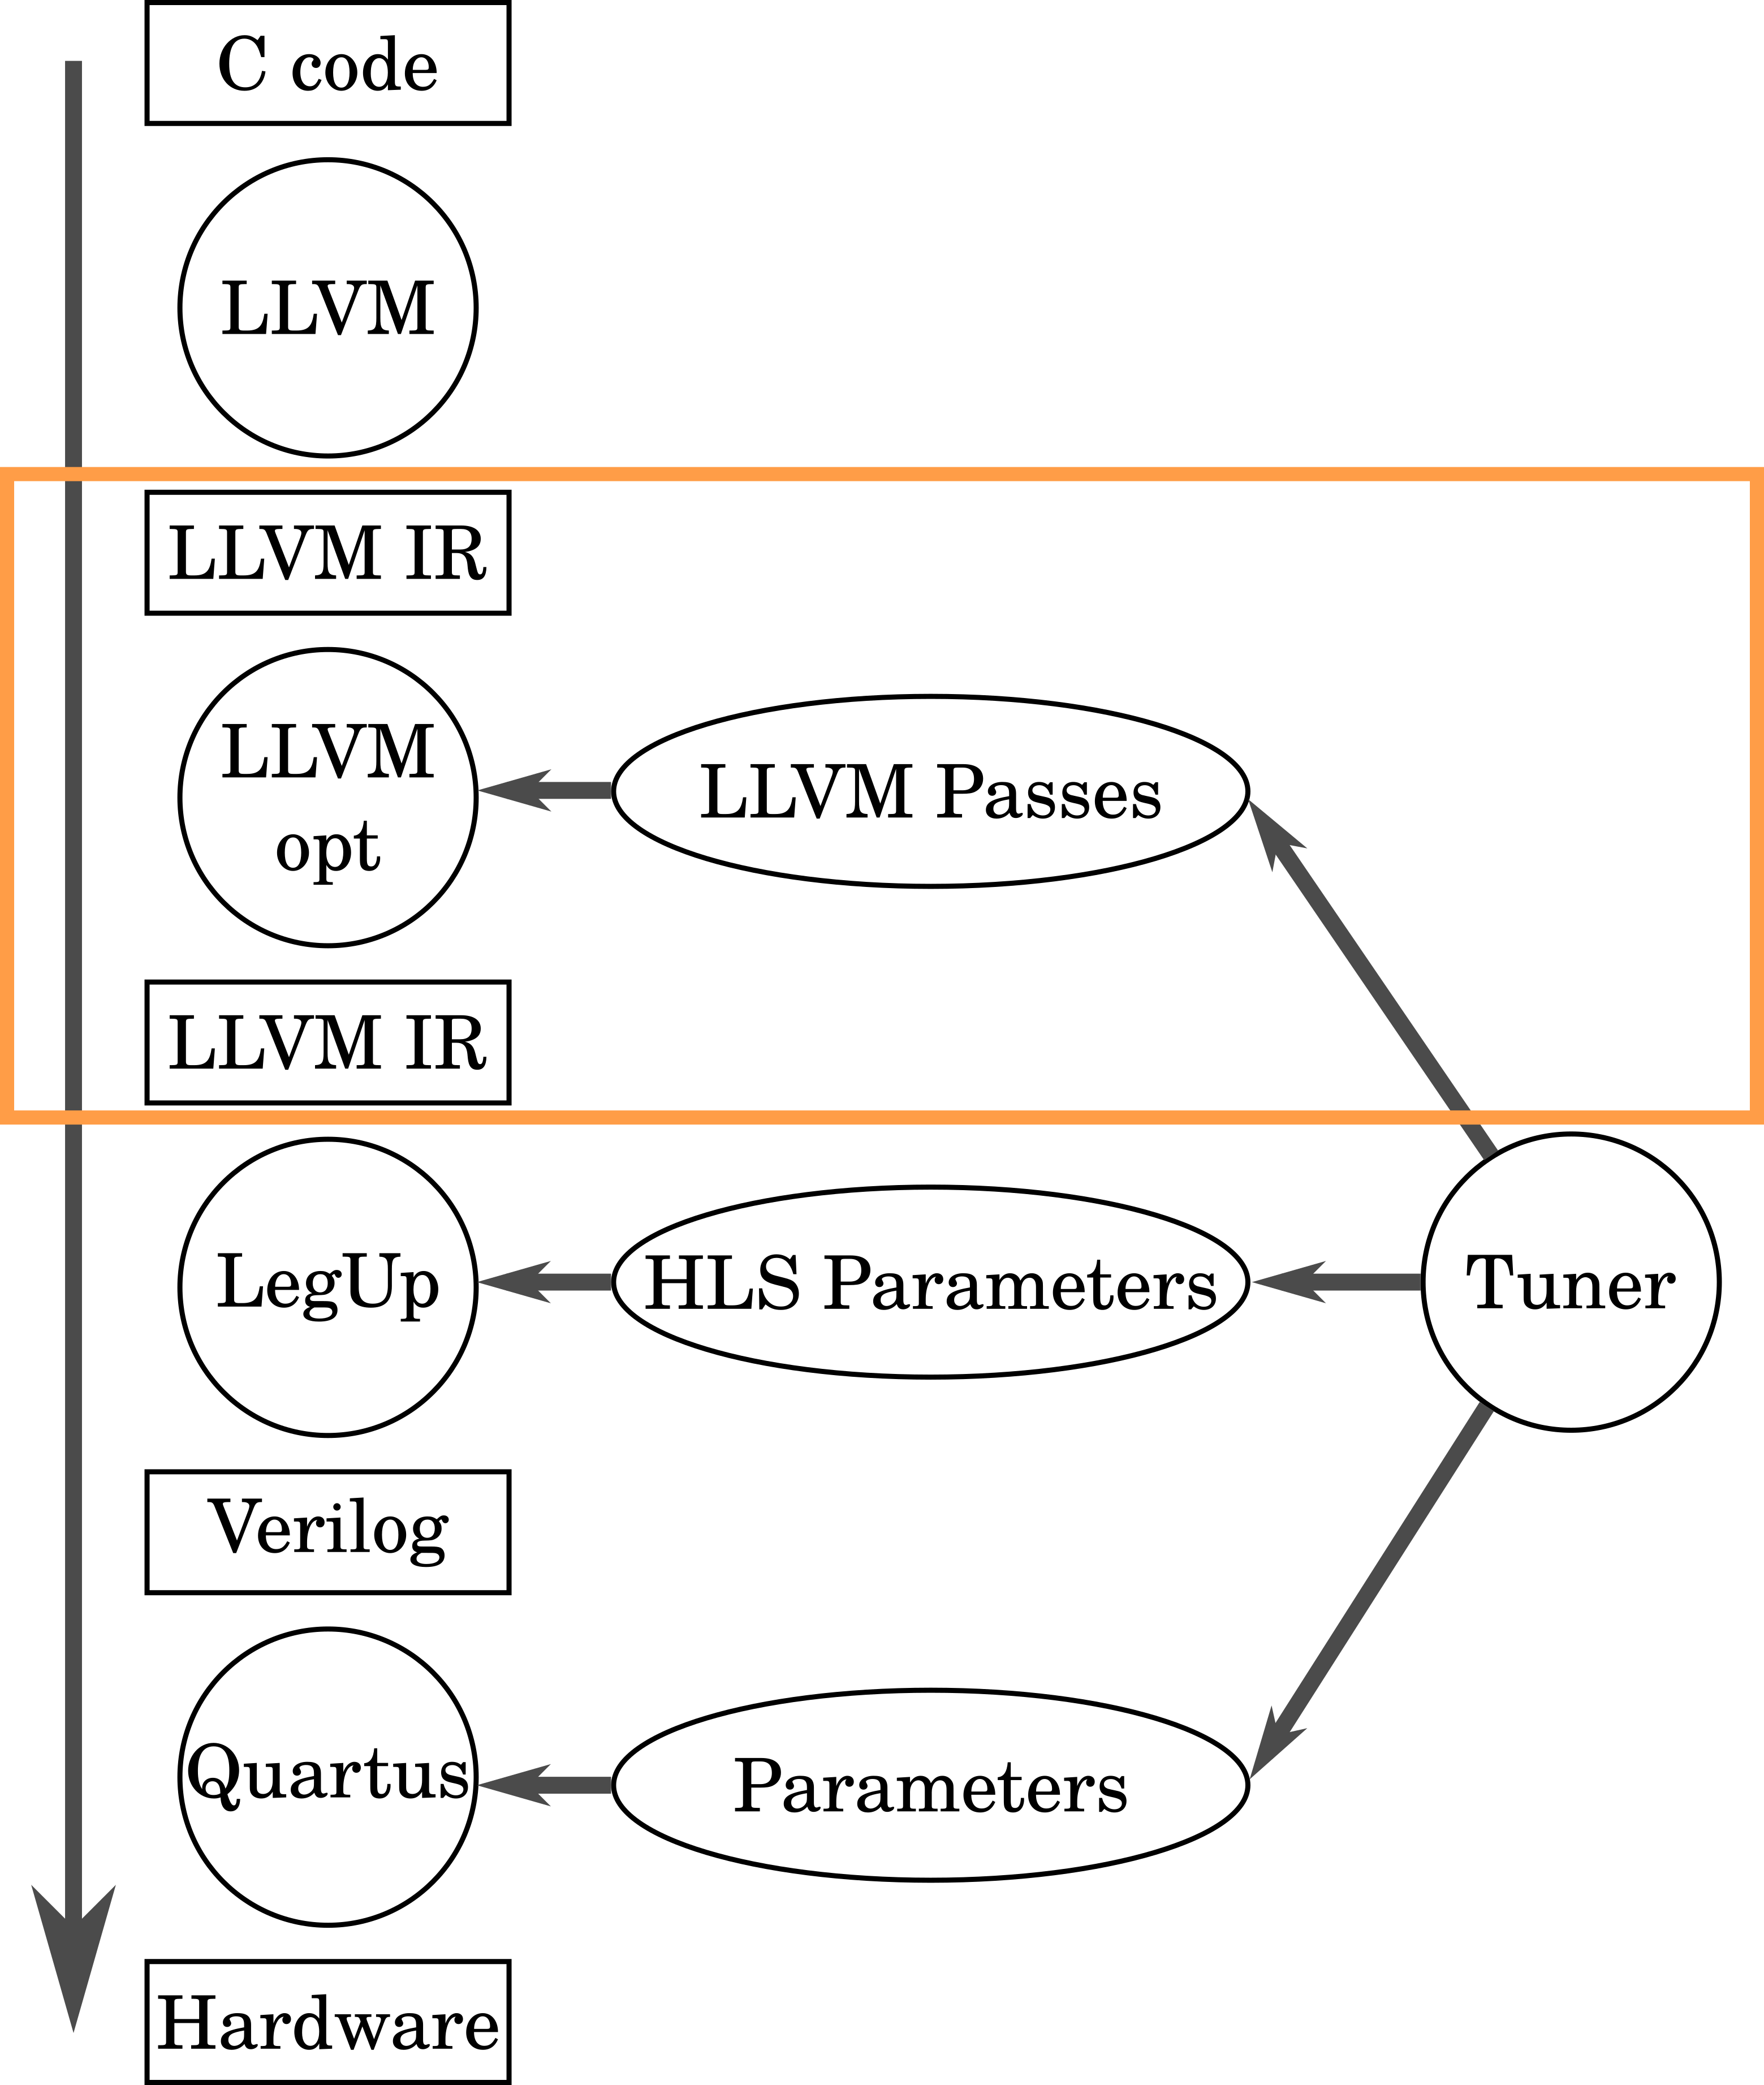
\includegraphics[width=.445\textwidth]{compile_flow_huang}
    \end{center}
\end{frame}

\begin{frame}
    \frametitle{Huang \textit{et al.}'s work}
    LLVM passes:
    \begin{itemize}
        \item Apply code \alert{optimizations} or \alert{transformations}
        \item \alert{Ordering} matters
        \item \texttt{-O3} is a specific \alert{set of passes}
        \item LegUp is implemented as a pass
    \end{itemize}

    Examples:
    \begin{itemize}
        \item \texttt{--dce}: Dead Code Elimination
        \item \texttt{--loop-extract}
        \item \texttt{--inline}
    \end{itemize}

    \begin{center}
        \tiny{Source: \url{llvm.org/docs/Passes.html} [Accessed on 15/09/16]}
    \end{center}
\end{frame}


\begin{frame}
    \frametitle{Comparison with Huang \textit{et al.}'s work}
    Our work:
    \begin{itemize}
        \item Selects \alert{LegUp's HLS} optimizations
        \item Targets the Cyclone V DE1-SoC
        \item Uses the \alert{CHStone benchmark}
        \item Performs \alert{Heuristic Search}
    \end{itemize}
\end{frame}

\begin{frame}
    \frametitle{Comparison with Huang \textit{et al.}'s work: Search Space}
    \begin{center}
        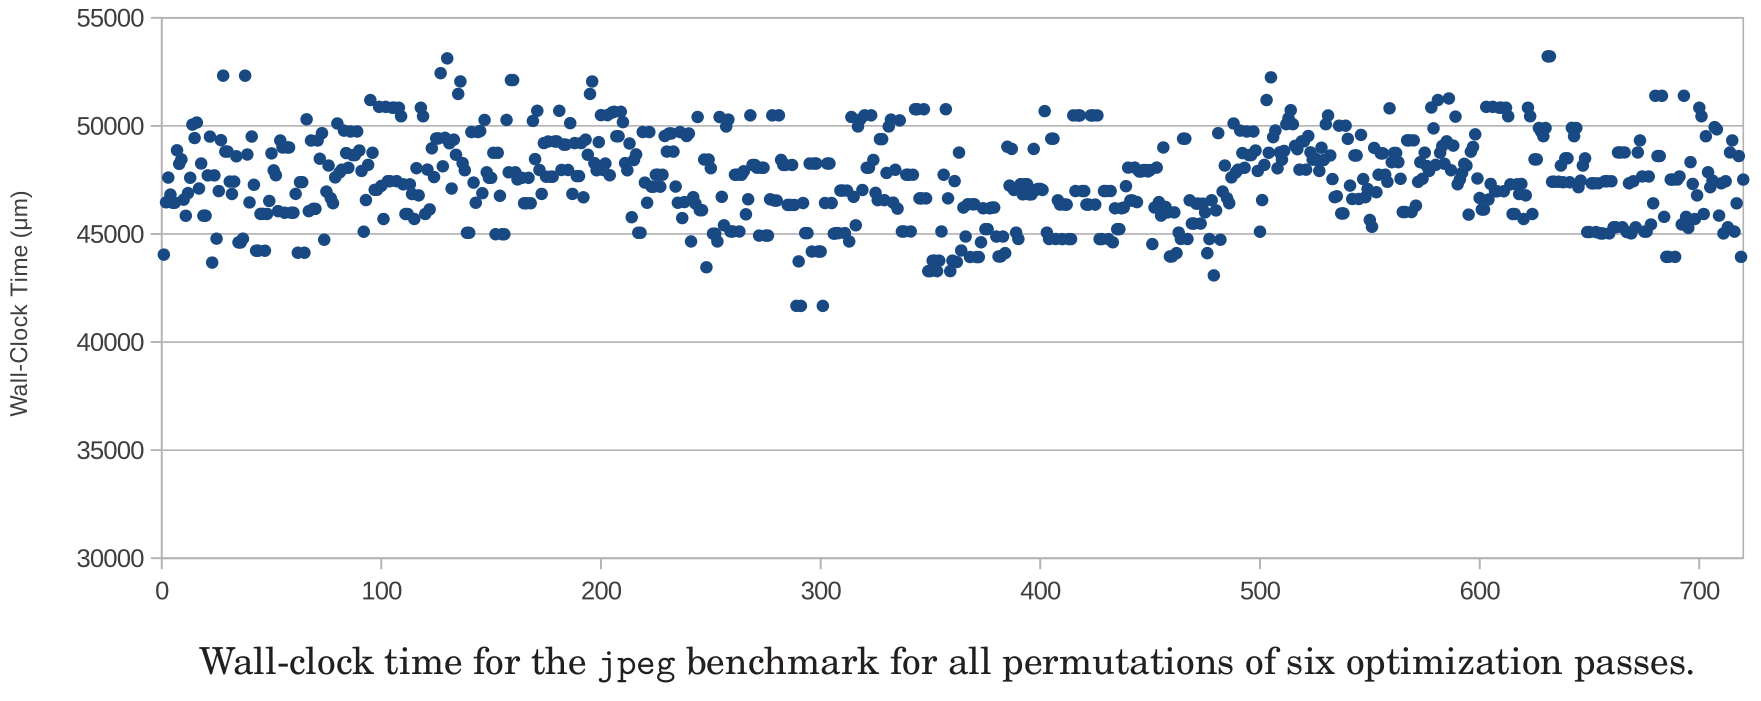
\includegraphics[width=.8\textwidth]{search_space}

        \tiny{Image: Huang, Qijing, et al. "The effect of compiler
        optimizations on high-level synthesis-generated hardware." ACM
        Transactions on Reconfigurable Technology and Systems (TRETS) 8.3
        (2015): 14.}
    \end{center}

    The LLVM flags search space:
    \begin{itemize}
        \item Abundance of \alert{Local Minima}
        \item \alert{Much smaller} than the HLS search space
    \end{itemize}
\end{frame}

\begin{frame}
    \frametitle{Comparison with Huang \textit{et al.}'s work}
    \begin{center}
        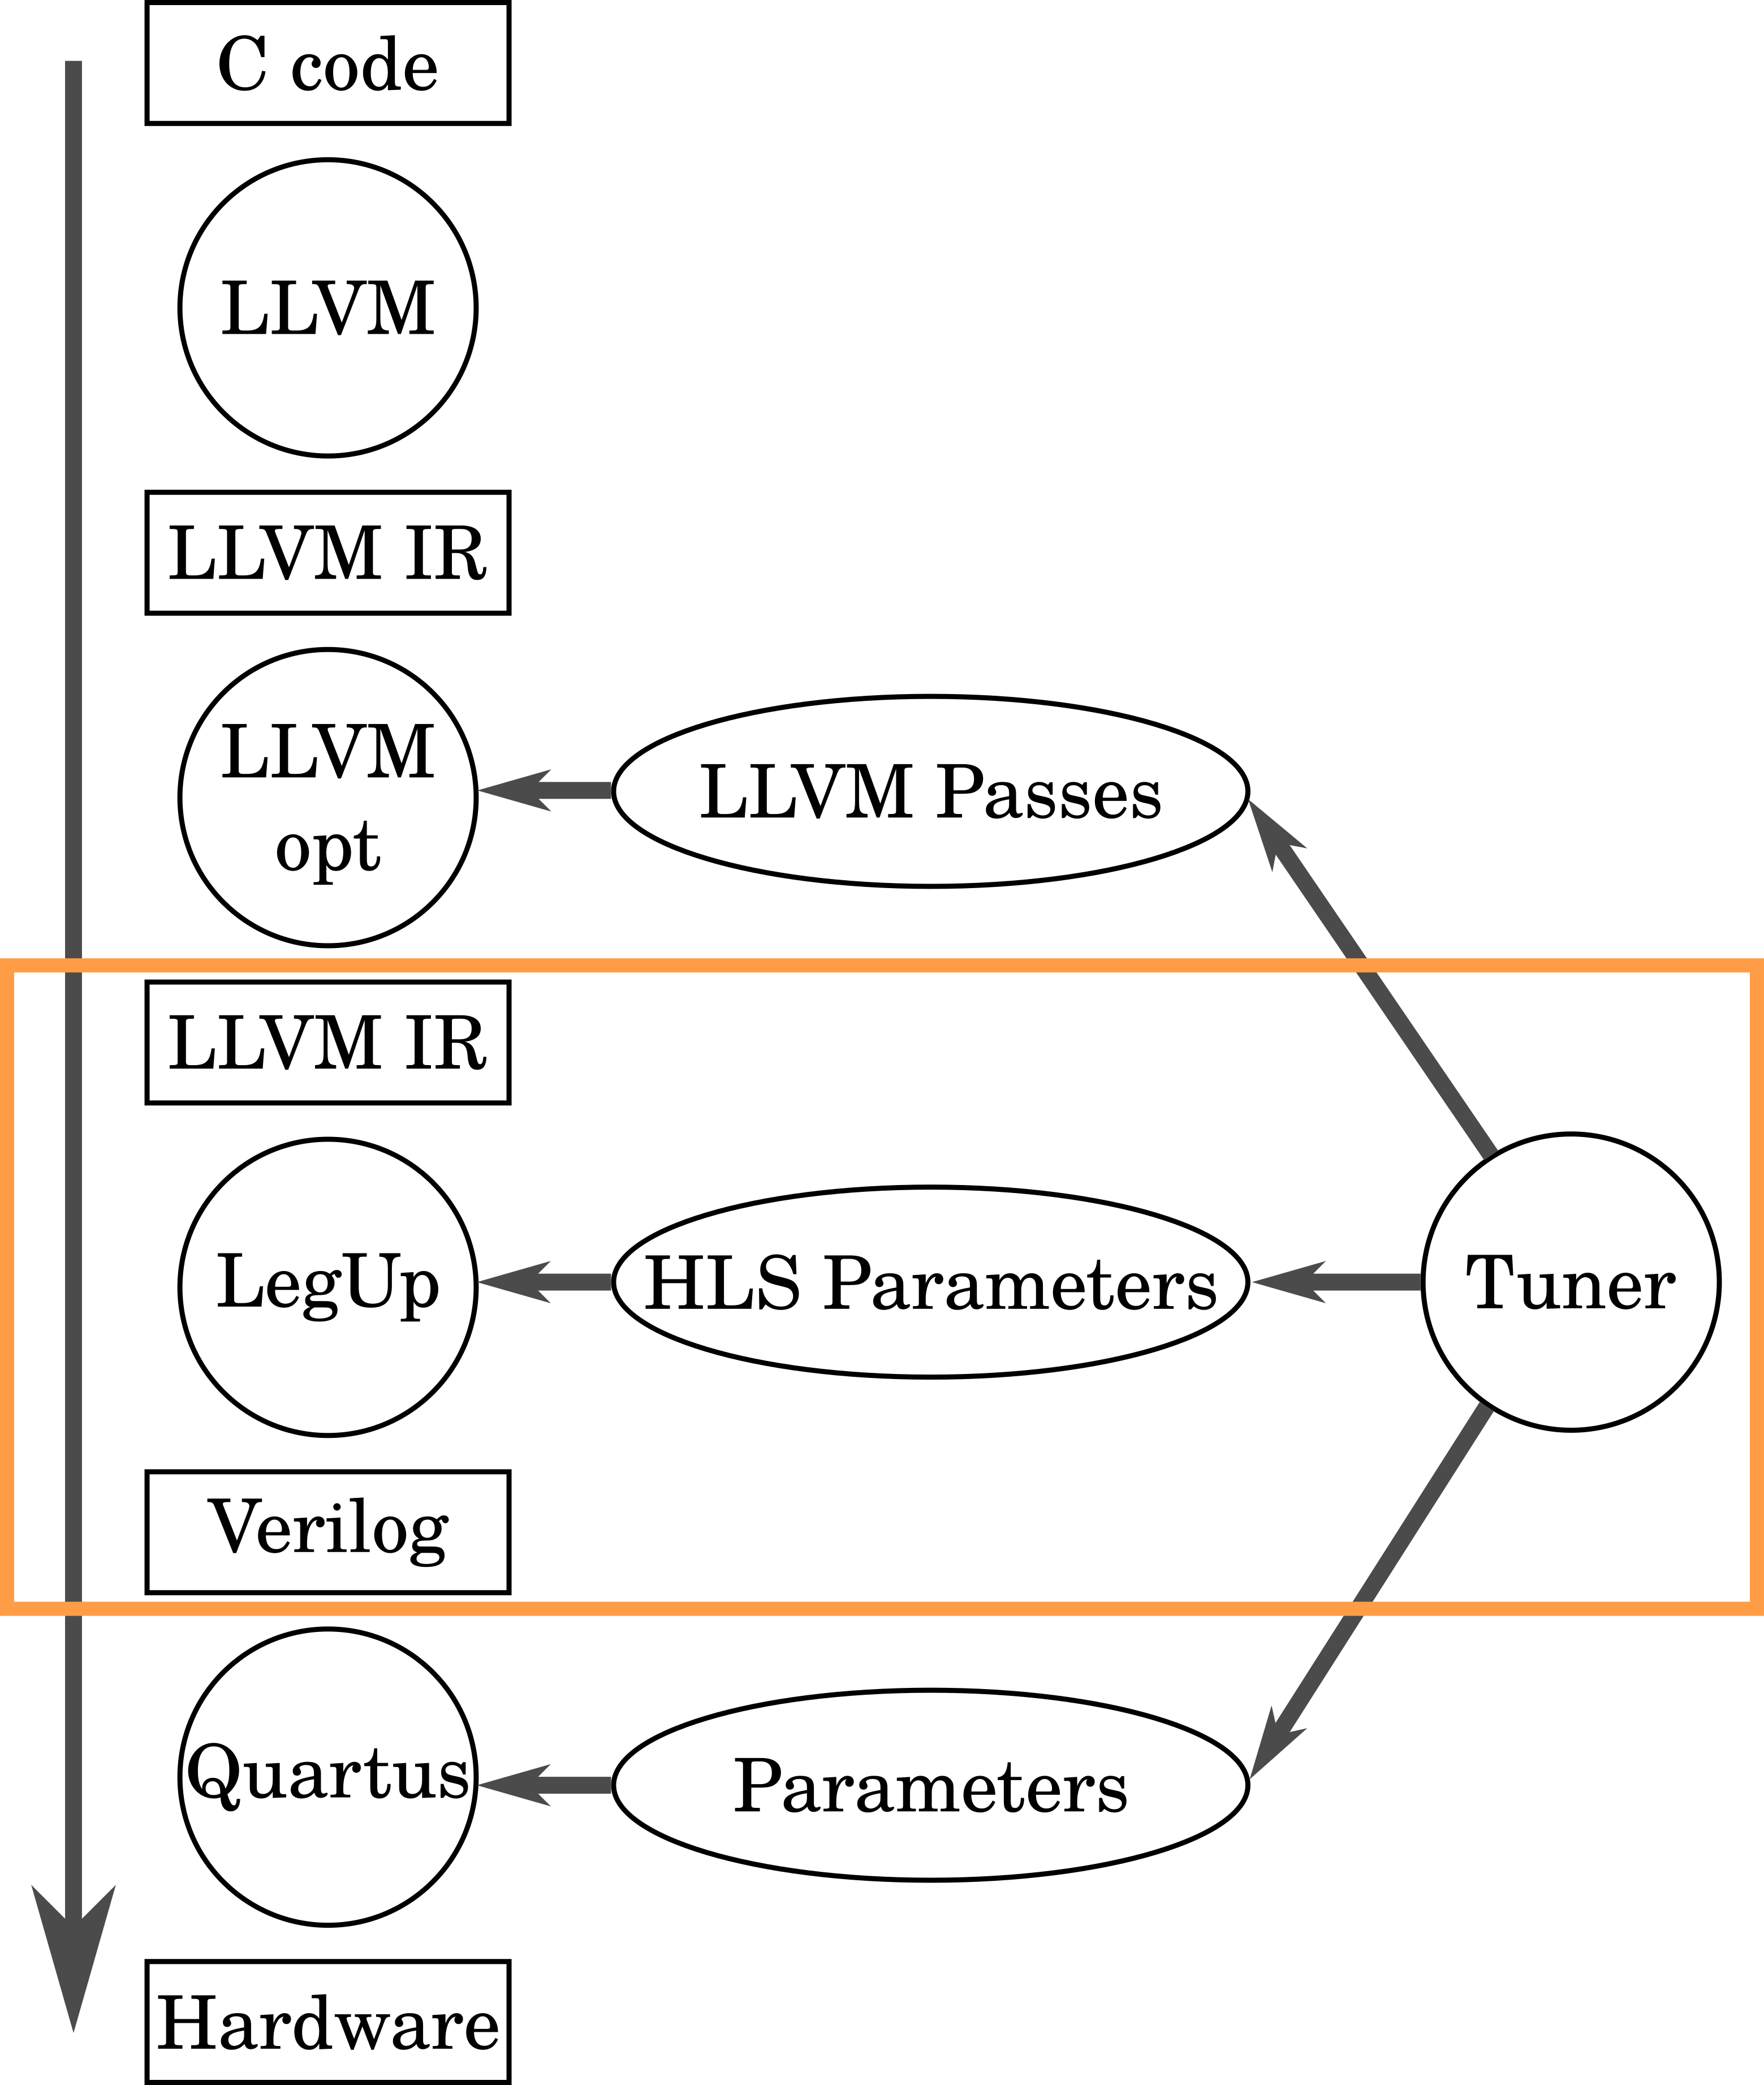
\includegraphics[width=.445\textwidth]{compile_flow_our}
    \end{center}
\end{frame}

\begin{frame}
    \frametitle{Comparison with Huang \textit{et al.}'s work: Wall-Clock Time}
    \begin{columns}[T]
        \column{.55\textwidth}
        \begin{center}
            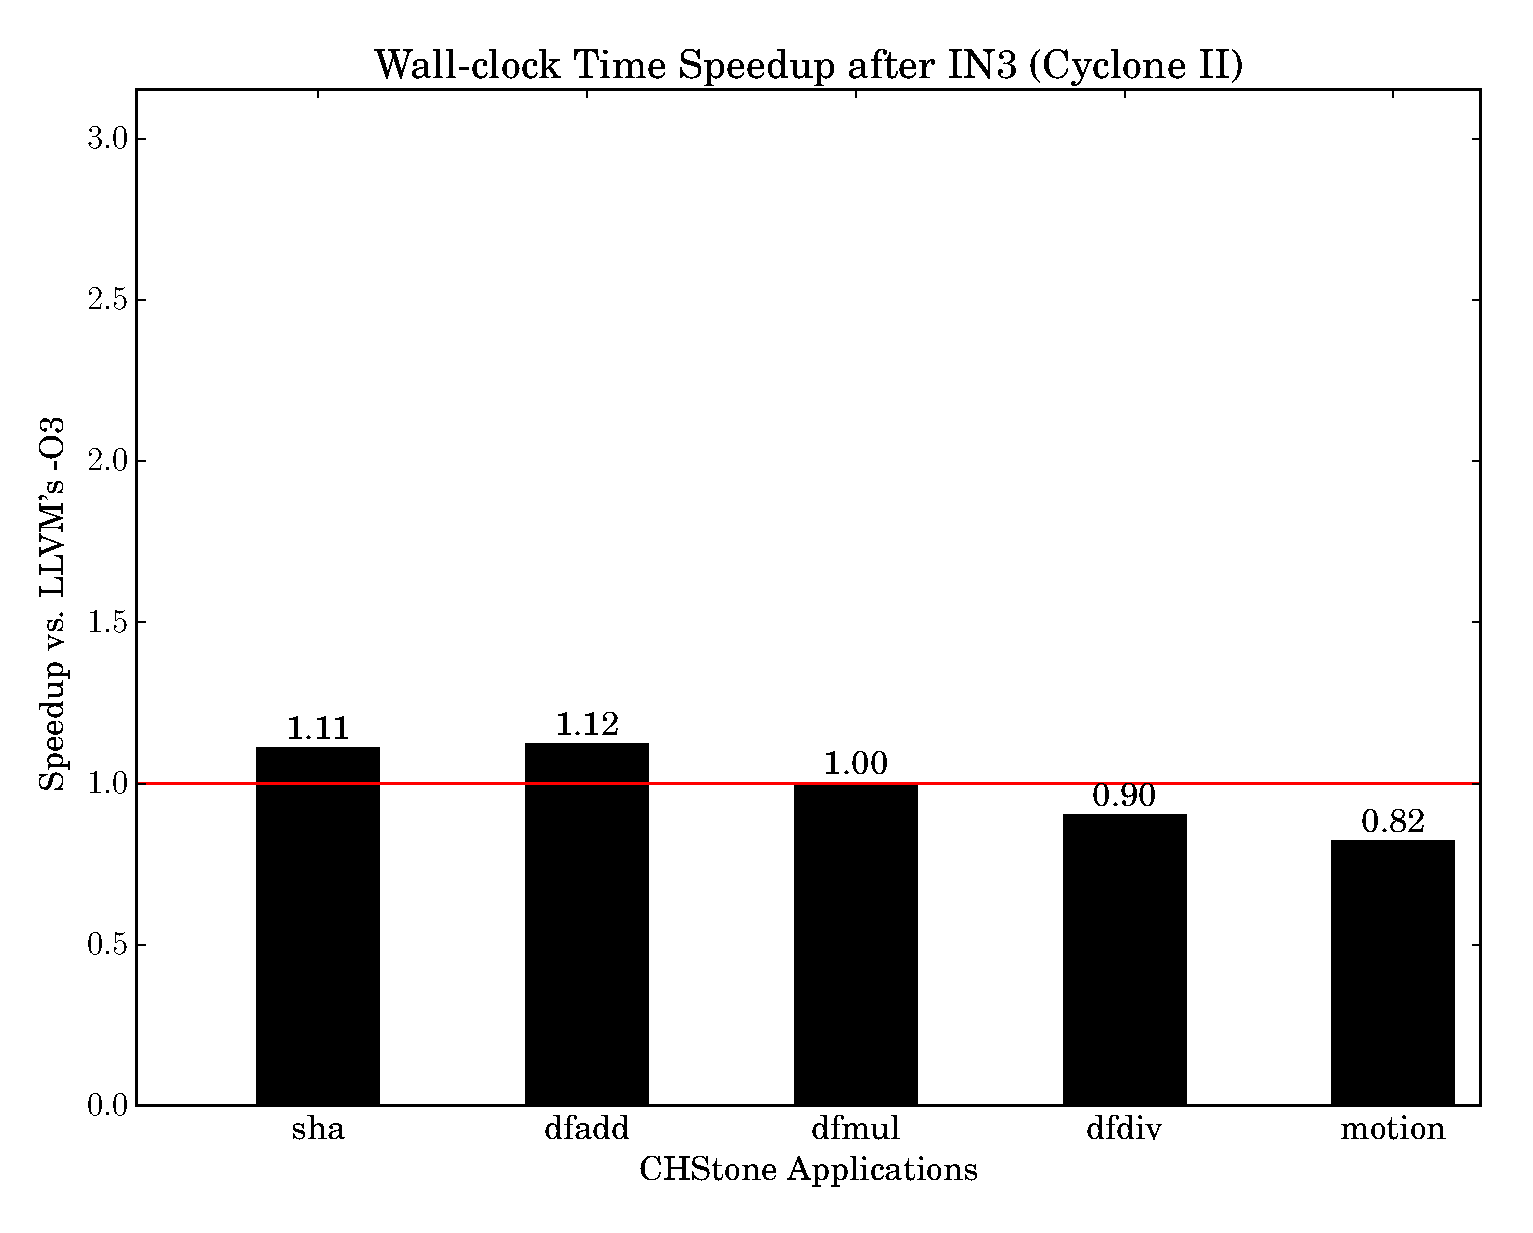
\includegraphics[width=\textwidth]{wct_speedups_chstone_IN3_llvm}
        \end{center}
        \column{.55\textwidth}
        \begin{center}
            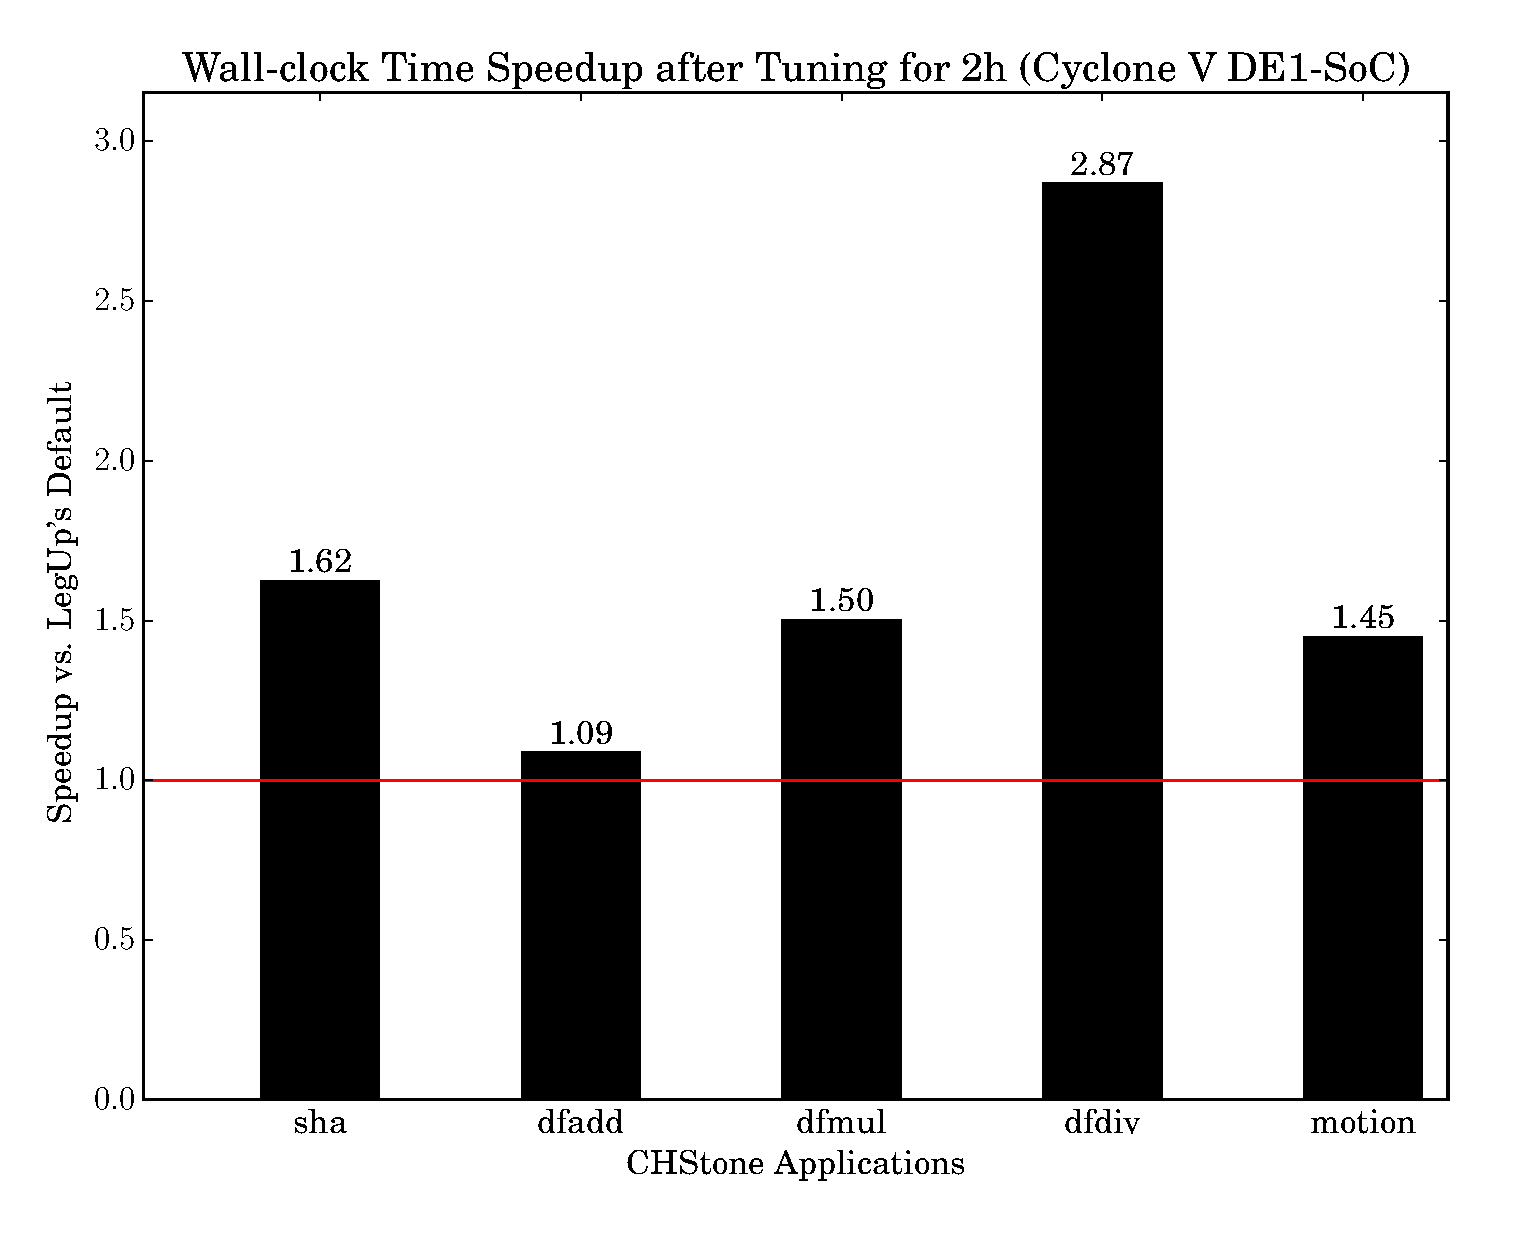
\includegraphics[width=\textwidth]{wct_speedups_chstone_7200_hls}
        \end{center}
    \end{columns}
\end{frame}

\begin{frame}
    \frametitle{Comparison with Huang \textit{et al.}'s work: Wall-Clock Time}
    \begin{center}
        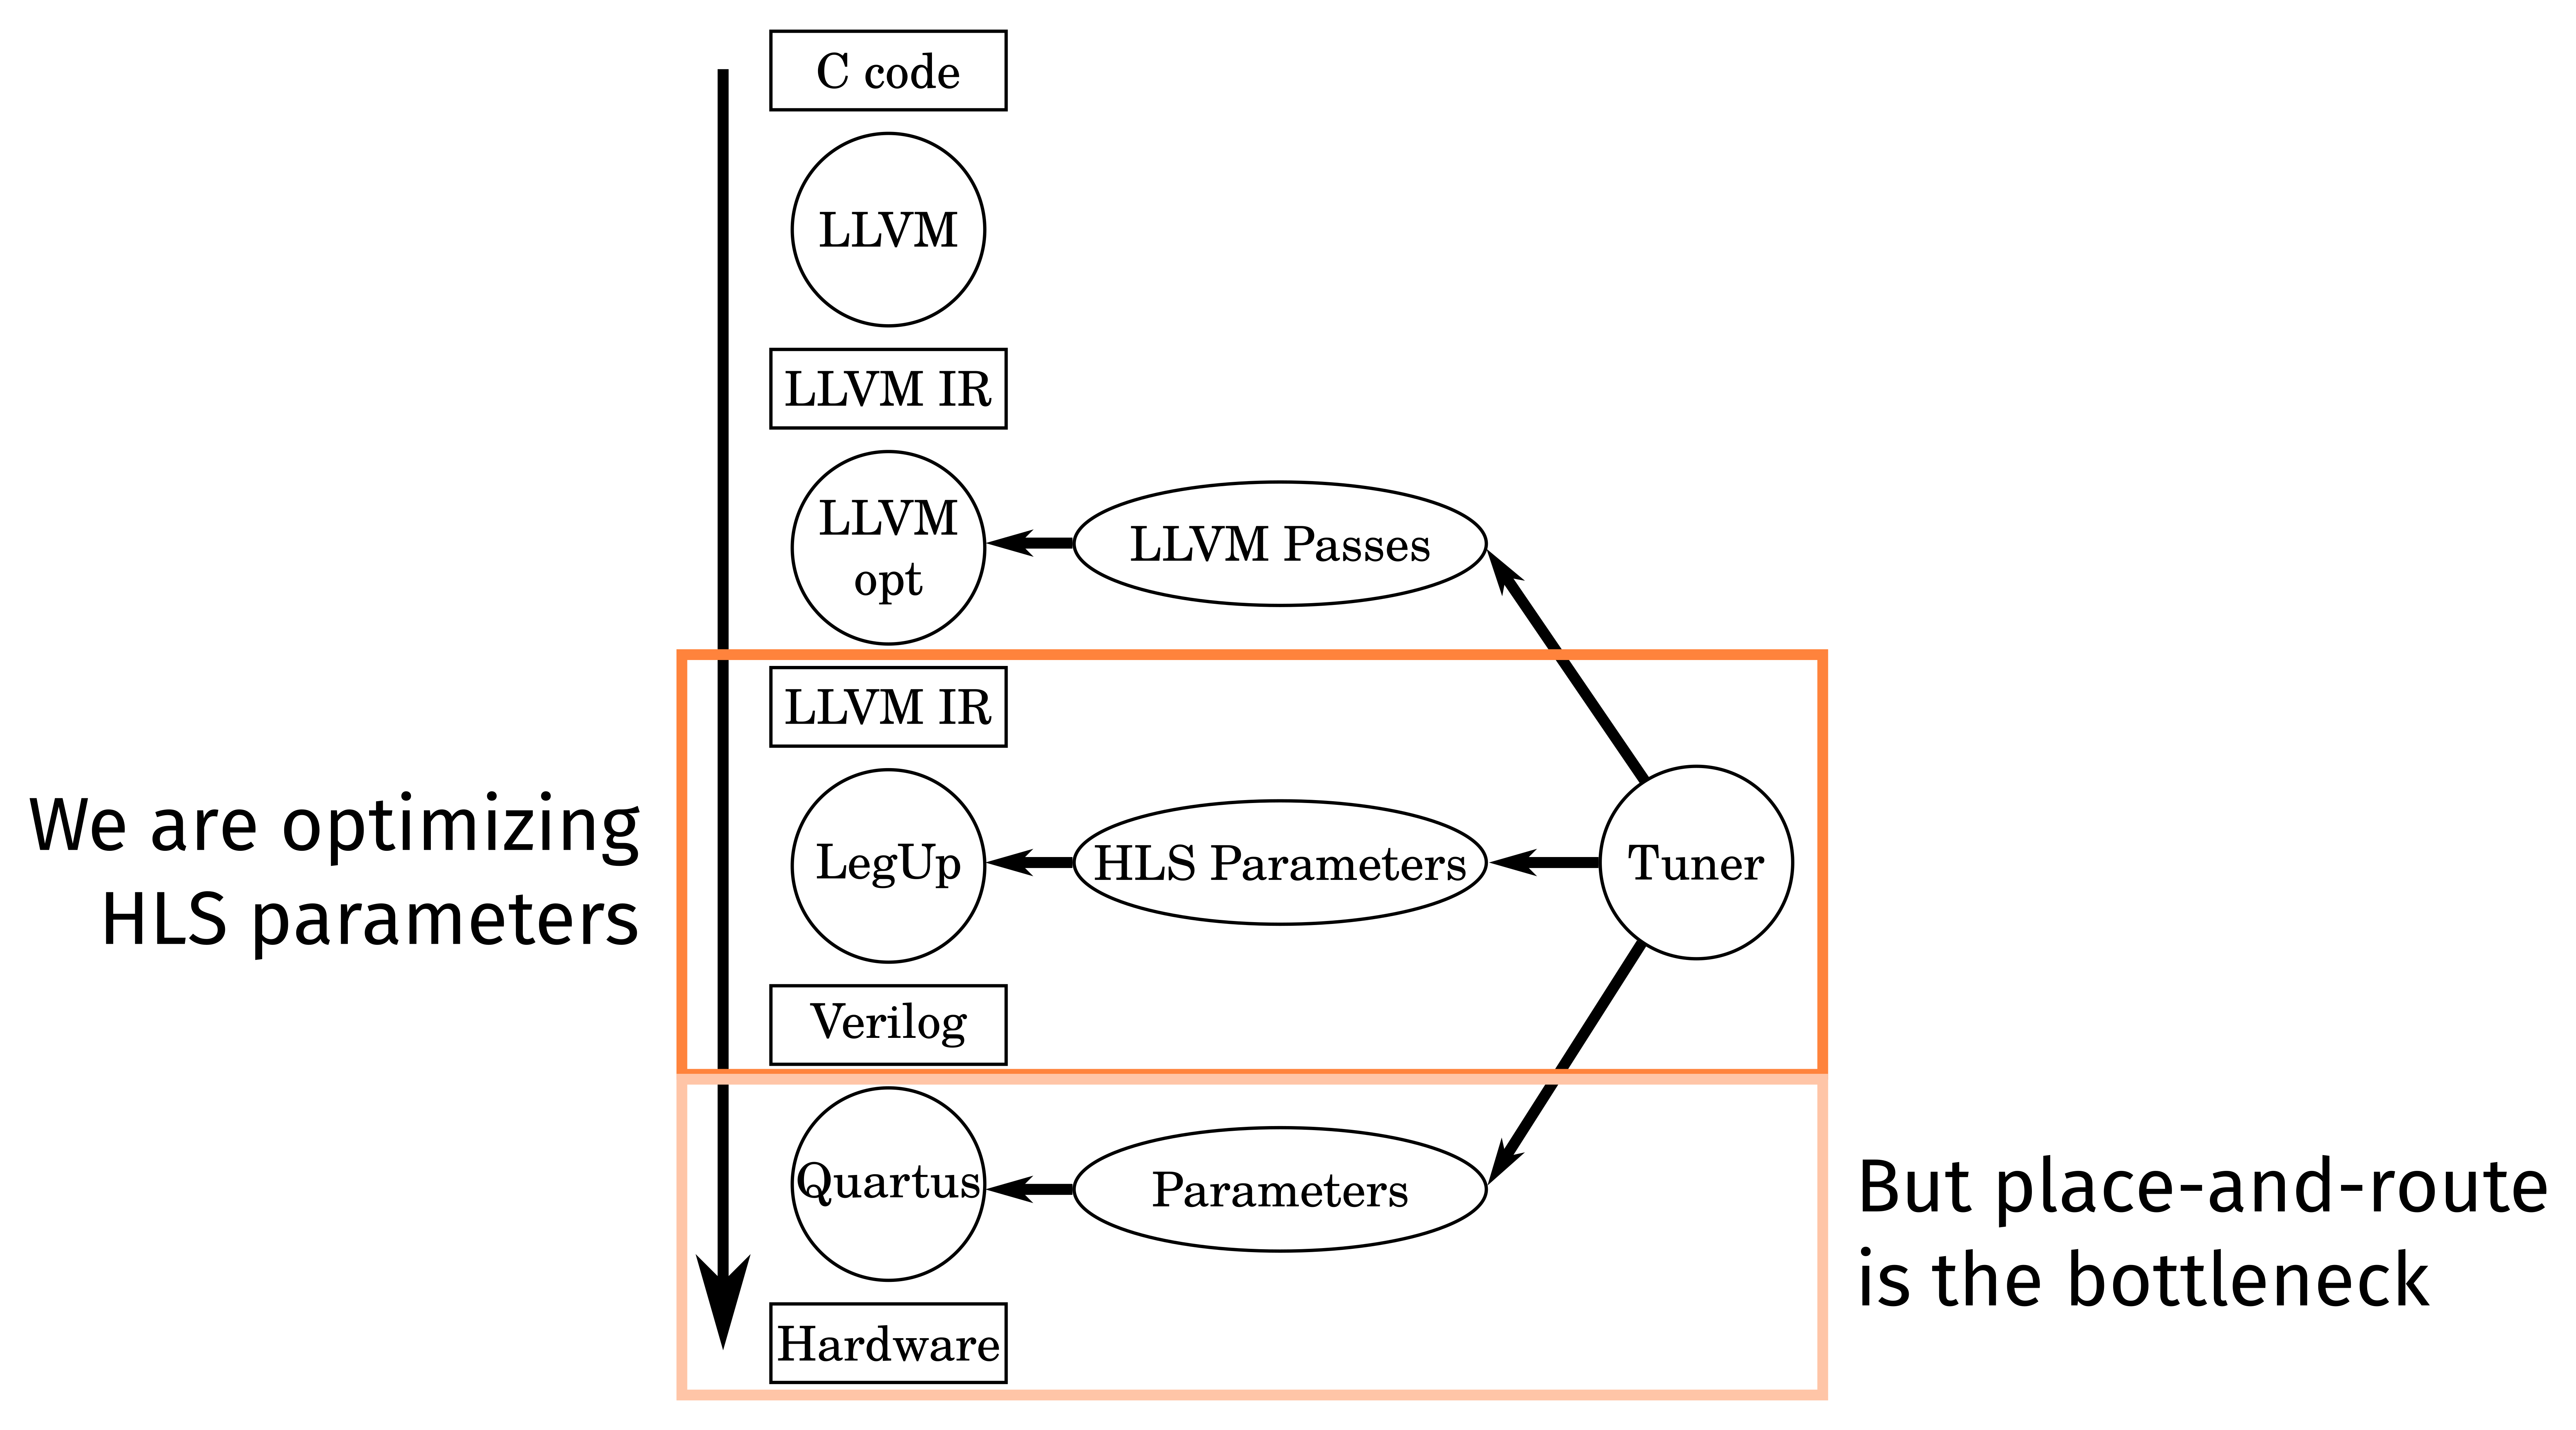
\includegraphics[width=.95\textwidth]{compile_flow_bottleneck_1}
    \end{center}
\end{frame}

\begin{frame}
    \frametitle{Comparison with Huang \textit{et al.}'s work: Clock Cycles}
    \begin{columns}[T]
        \column{.55\textwidth}
        \begin{center}
            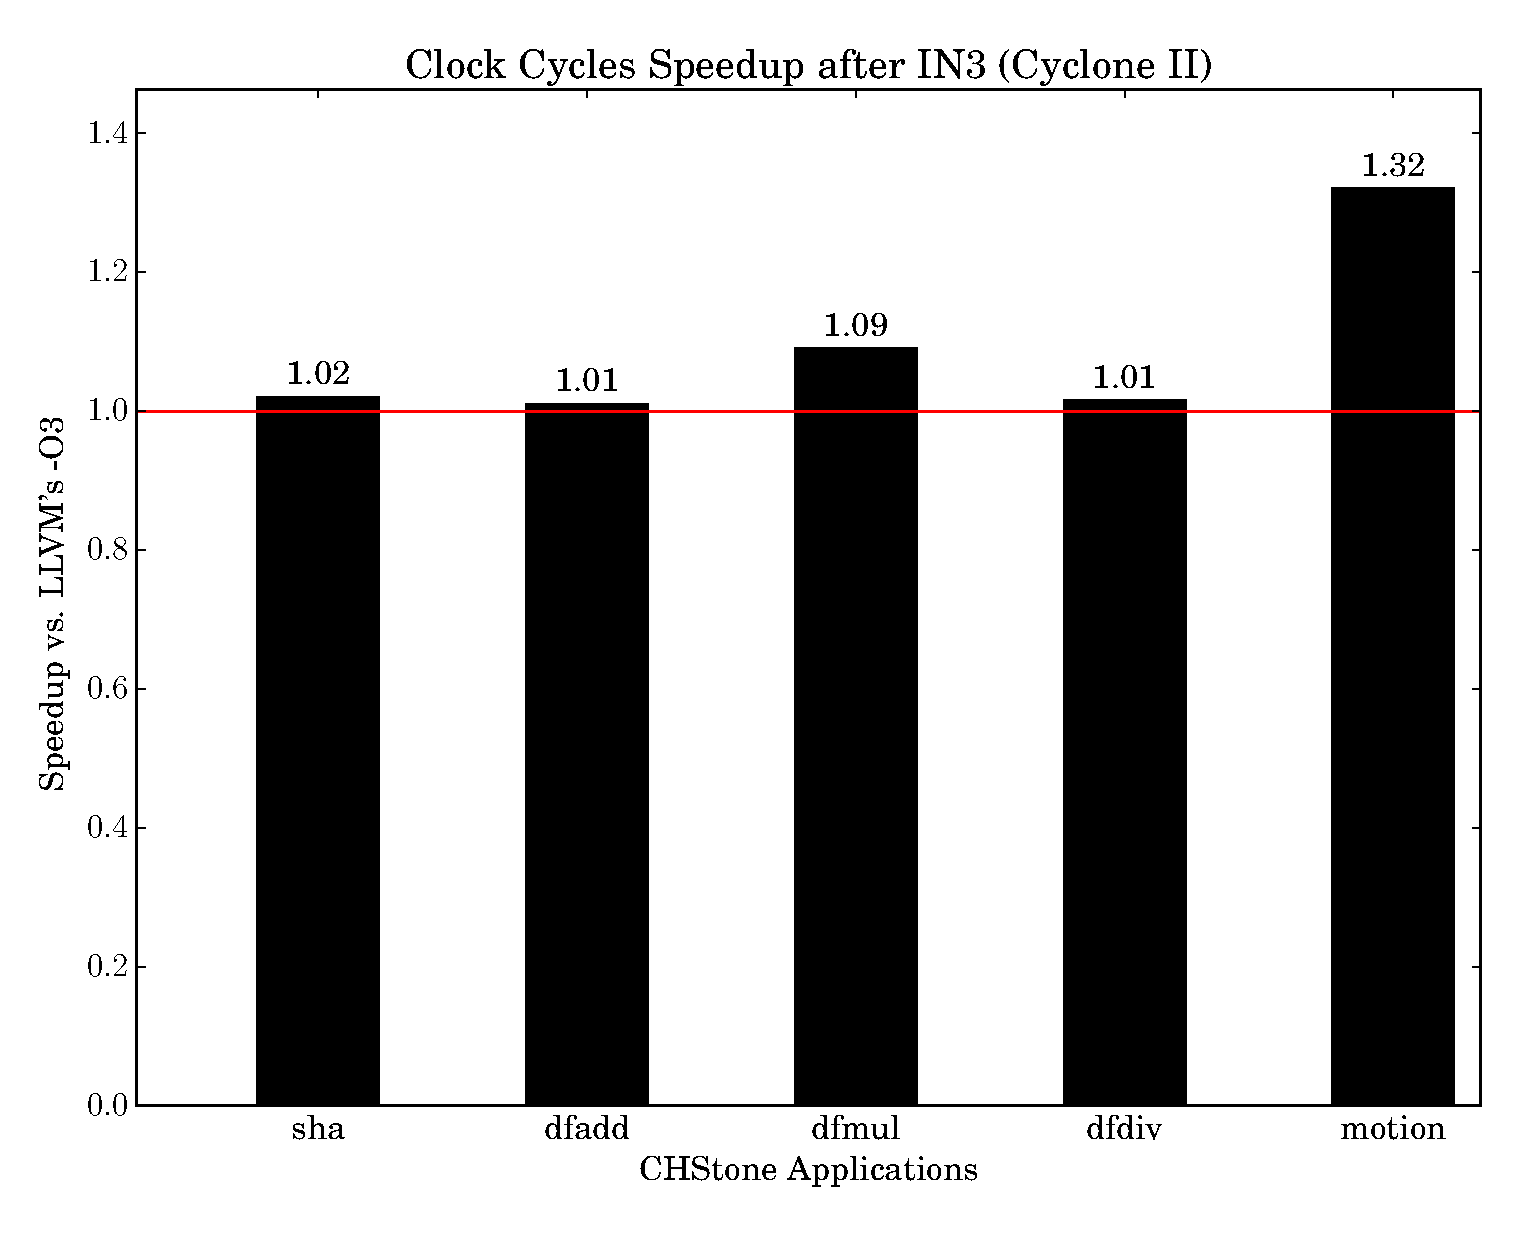
\includegraphics[width=\textwidth]{clk_speedups_chstone_IN3_llvm}
        \end{center}
        \column{.55\textwidth}
        \begin{center}
            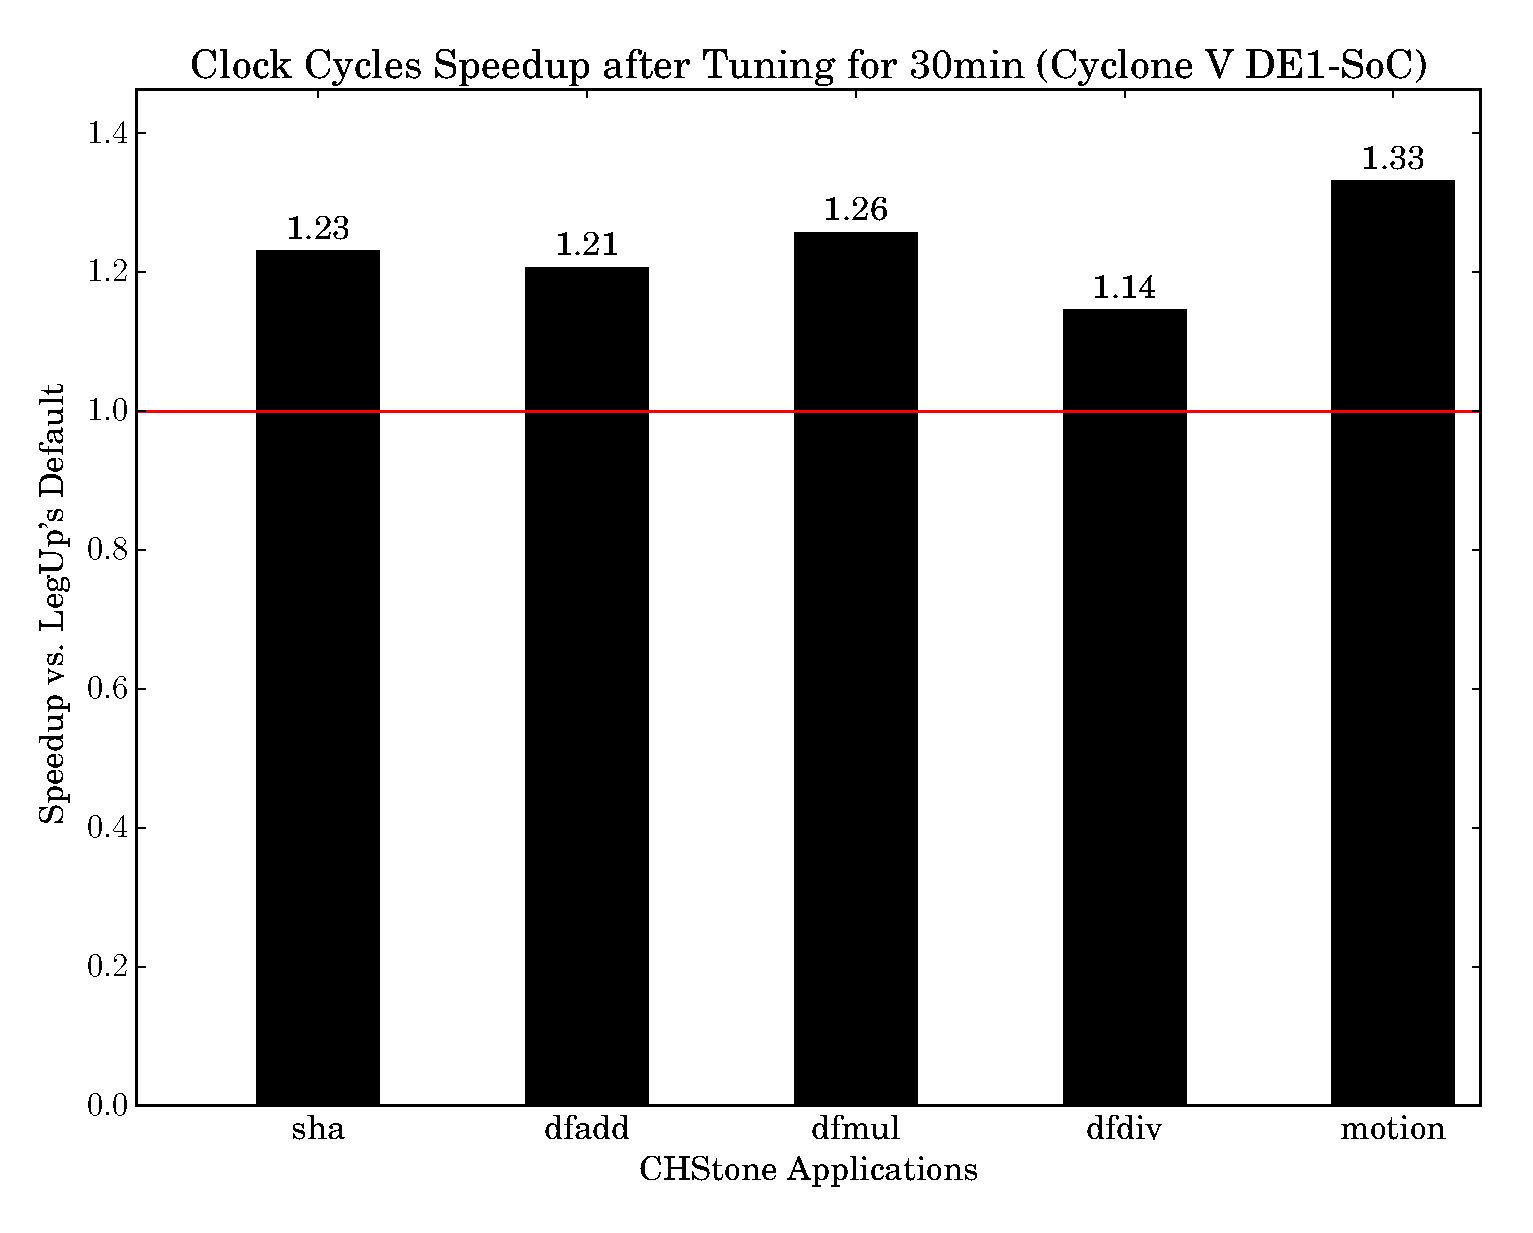
\includegraphics[width=\textwidth]{clk_speedups_chstone_1800_hls}
        \end{center}
    \end{columns}
\end{frame}

\begin{frame}
    \frametitle{Comparison with Huang \textit{et al.}'s work: Conclusion}
    \begin{itemize}
        \item We optimized \alert{LegUp's HLS parameters}
        \item Huang \textit{et al.} optimized \alert{LLVM's passes}
        \item Targeted \alert{different FPGAs}
        \item Achieved similar speedup magnitude
        \item Huang \textit{et al.} does not report time to achieve results
    \end{itemize}
\end{frame}

\begin{frame}
    \frametitle{Next Steps}
    \begin{itemize}
        \item More \alert{complex benchmarks}: Rodinia OpenMP, OpenDwarfs
        \item Autotuning with \alert{OpenCL HLS} tools
        \item Optimize parameters from \alert{different HLS steps}
        \item Use a \alert{cost model} to improve autotuning performance
        \item \alert{Parallel and distributed} autotuning
    \end{itemize}
\end{frame}

\begin{frame}
    \frametitle{Next Steps: Combining Optimizations}
    \begin{center}
        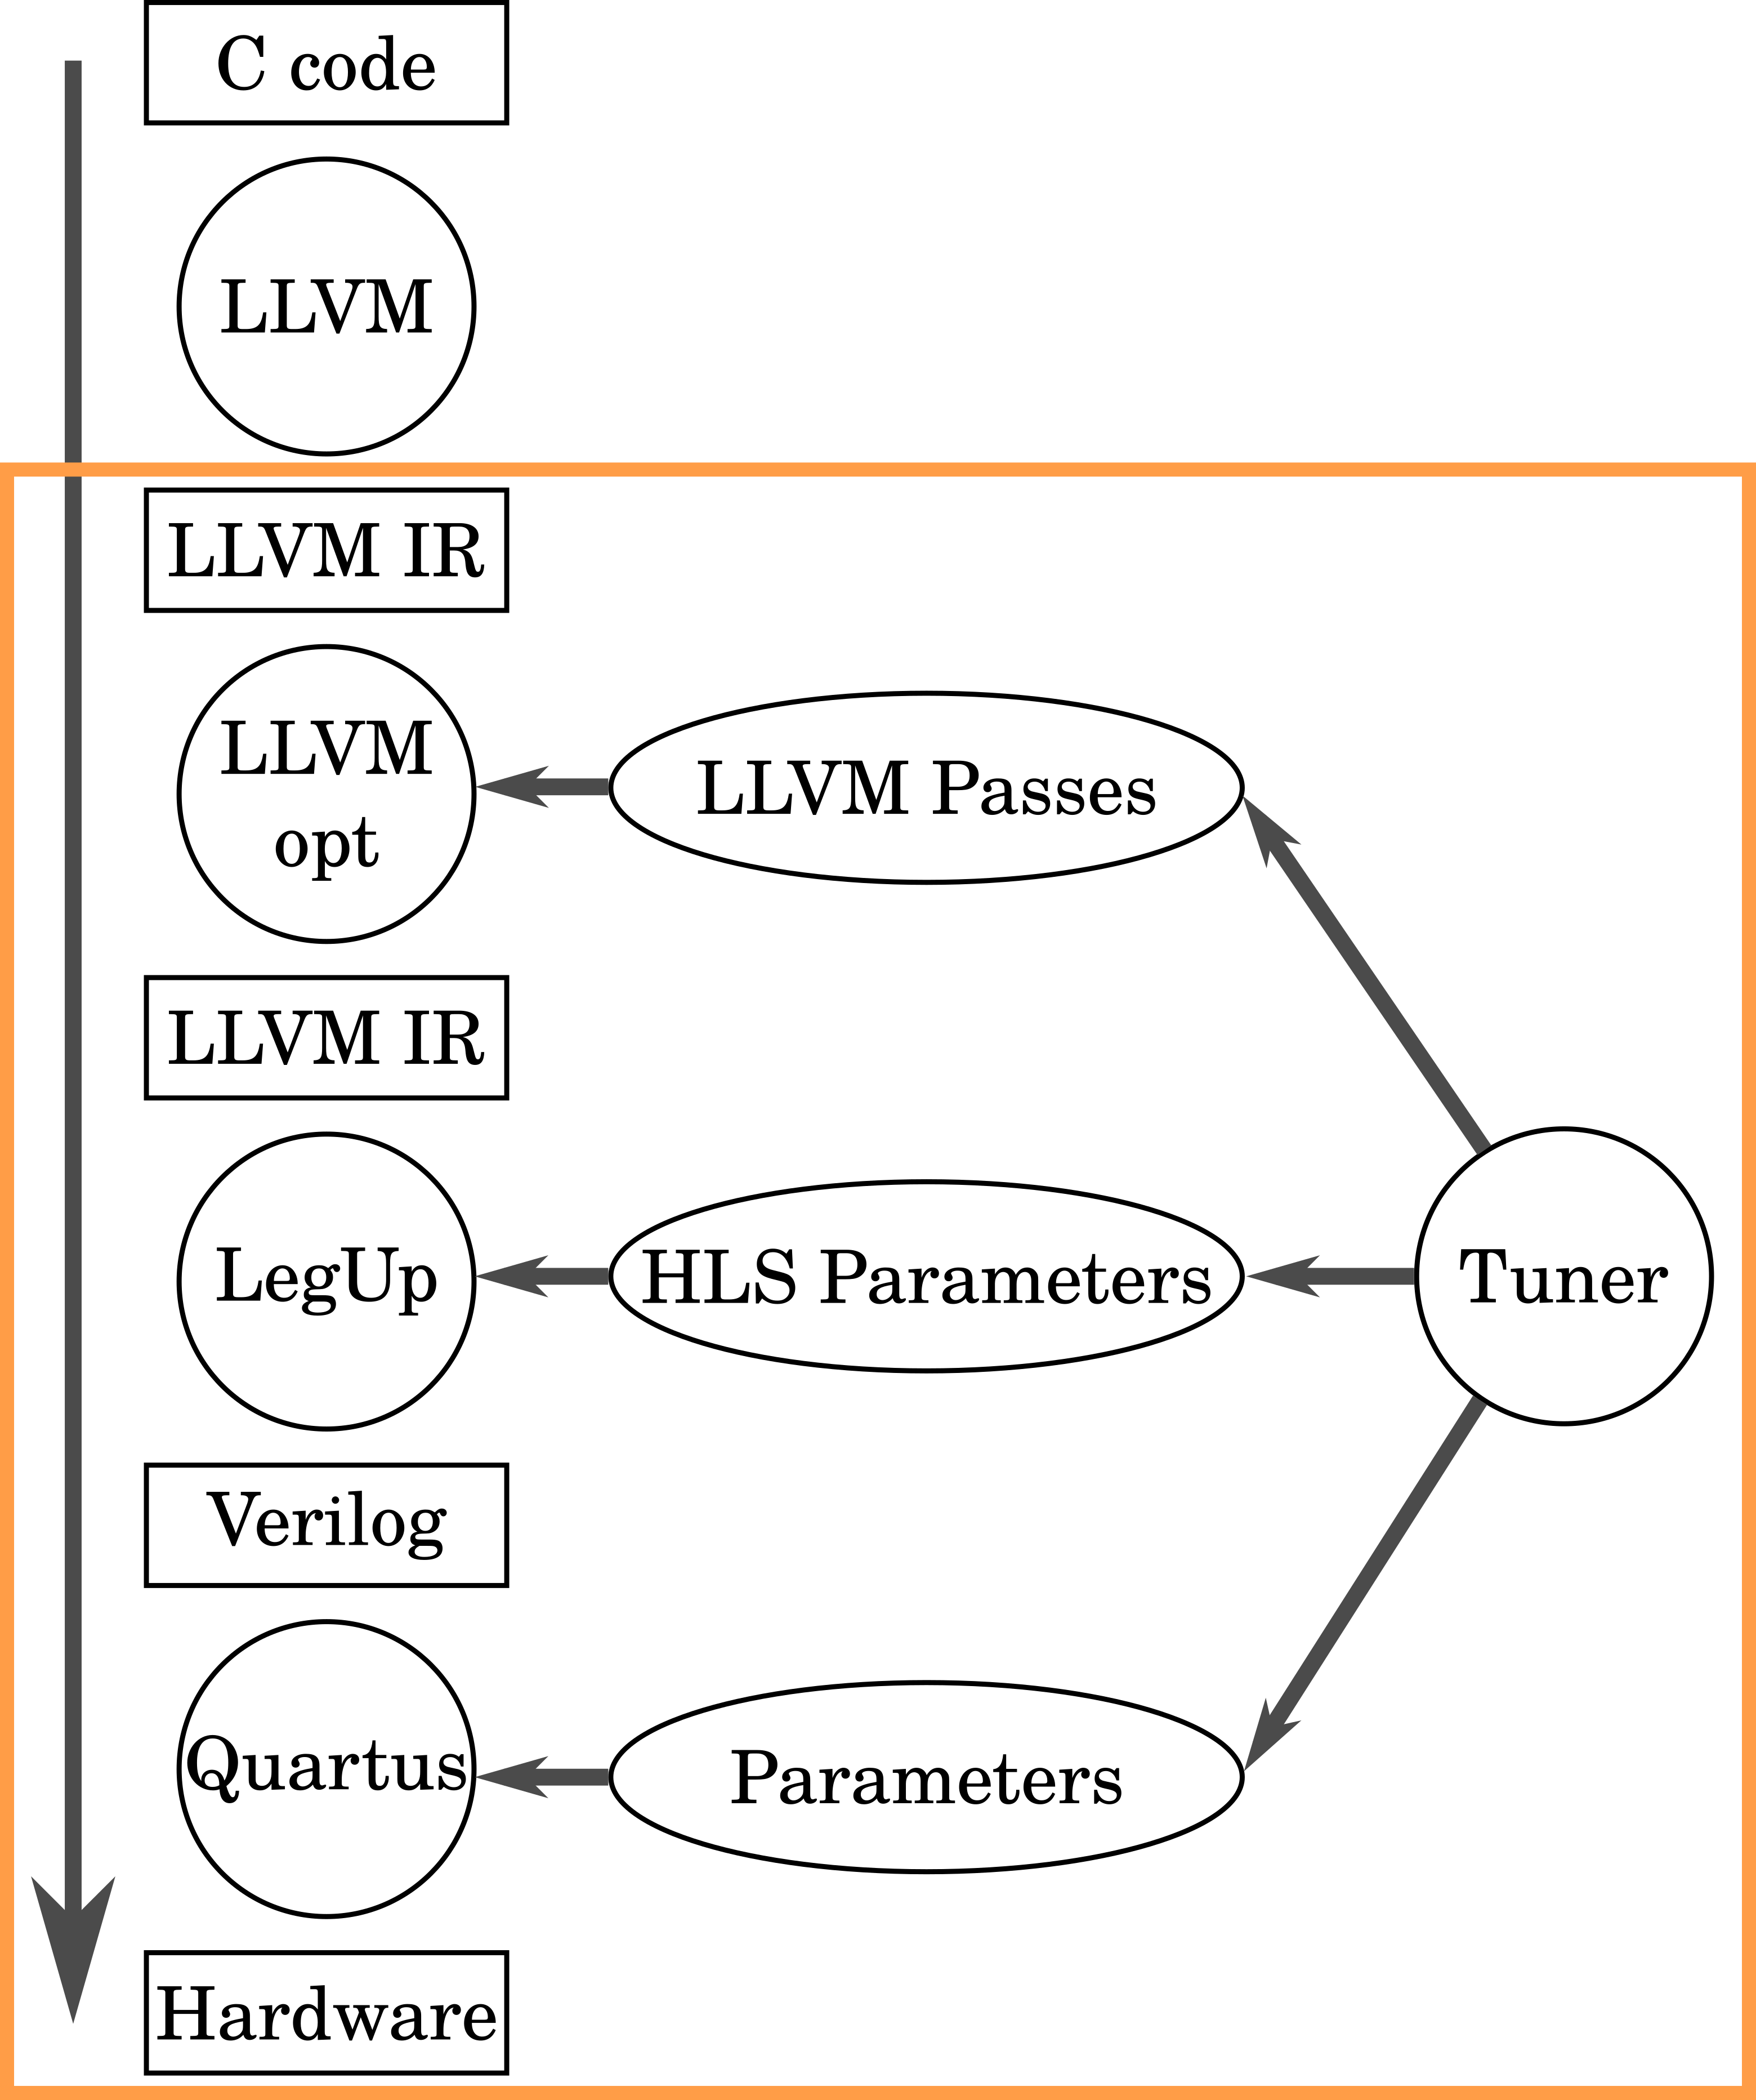
\includegraphics[width=.445\textwidth]{compile_flow_possible}
    \end{center}
\end{frame}

\begin{frame}
    \frametitle{Next Steps: Using a Cost Model}
    Using LegUp’s \alert{resource estimation} reports:
    \begin{itemize}
        \item Testing each configuration takes \alert{only a few seconds}
        \item Cost function:
    \end{itemize}
    \begin{align*}
    (w_1 \cdot Fmax) + (w_2 \cdot CombinatorialLEs) + (w_3 \cdot Registers) + (w_4 \cdot DSPs) + (w_5 \cdot Op1) + \dots
    \end{align*}

    \alert{Problem}: LegUp estimates resources \alert{too early} (during Allocation):
    \begin{itemize}
        \item Estimate is obtained  \alert{before all HLS optimizations}
        \item Is it possible to estimate later?
    \end{itemize}
\end{frame}

\begin{frame}
    \frametitle{Next Steps: Parallel and Distributed Autotuning}
    \begin{center}
        
\includegraphics[width=.75\textwidth]{stochasticsearch_logo}
    \end{center}

    We are working on an autotuning framework:
    \begin{itemize}
        \item In the \alert{Julia} language
        \item High-Level abstractions
        \item Parallel and distributed autotuning
        \item \url{github.com/phrb/StochasticSearch.jl}
    \end{itemize}
\end{frame}

\maketitle

\end{document}
